\documentclass{extbook}[14pt]
\usepackage{multicol, enumerate, enumitem, hyperref, color, soul, setspace, parskip, fancyhdr, amssymb, amsthm, amsmath, latexsym, units, mathtools}
\everymath{\displaystyle}
\usepackage[headsep=0.5cm,headheight=0cm, left=1 in,right= 1 in,top= 1 in,bottom= 1 in]{geometry}
\usepackage{dashrule}  % Package to use the command below to create lines between items
\newcommand{\litem}[1]{\item #1

\rule{\textwidth}{0.4pt}}
\pagestyle{fancy}
\lhead{}
\chead{Answer Key for CRIF Functions 8 Version ALL}
\rhead{}
\lfoot{1542-4749}
\cfoot{}
\rfoot{test}
\begin{document}
\textbf{This key should allow you to understand why you choose the option you did (beyond just getting a question right or wrong). \href{https://xronos.clas.ufl.edu/mac1105spring2020/courseDescriptionAndMisc/Exams/LearningFromResults}{More instructions on how to use this key can be found here}.}

\textbf{If you have a suggestion to make the keys better, \href{https://forms.gle/CZkbZmPbC9XALEE88}{please fill out the short survey here}.}

\textit{Note: This key is auto-generated and may contain issues and/or errors. The keys are reviewed after each exam to ensure grading is done accurately. If there are issues (like duplicate options), they are noted in the offline gradebook. The keys are a work-in-progress to give students as many resources to improve as possible.}

\rule{\textwidth}{0.4pt}

\begin{enumerate}\litem{
Is the graph below a linear function?

\begin{center}
    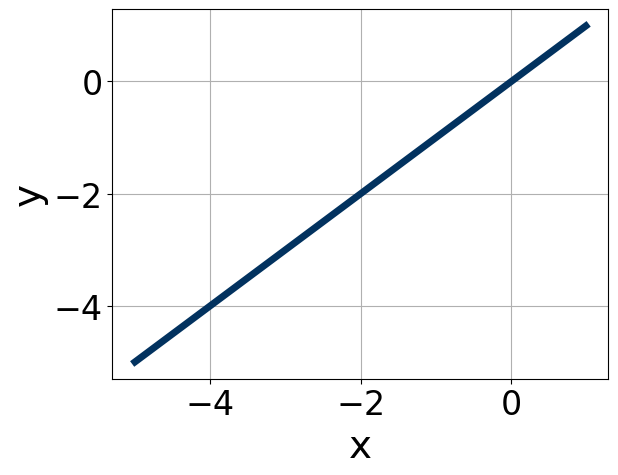
\includegraphics[width=0.5\textwidth]{../Figures/MA_8_F_1_2_graphA.png}
\end{center}


The solution is yes, the graph is linear., which is option A.

\begin{enumerate}[label=\Alph*.]
\item Yes, the graph is linear

* Correct! The graph has a constant rate of change and is thus a linear function.
\item No, the graph is not linear.

A linear function has a constant rate of growth. As $x$ increases/decreases, $y$ increases/decreases at the same rate. The graph in this example does have a constant rate of change.
\end{enumerate}


\textbf{General Comment:} The equation graphed was 1(x + 2)-2. A linear function has a constant rate of growth. This means that as $x$ increases or decreases, $y$ increase or decreases at the same rate. For example, $x^2$ is NOT a linear function. As $x$ increases, the $y$ increases faster and faster. From $x=1$ to $x=2$, the $y$ increases by 3. From $x=2$ to $x=3$, the $y$ increases by 5. From $x=3$ to $x=4$, the $y$ increases by 7. A linear function would have the same change in $y$ for any change in $x$.
}
\litem{
Is the following relation a function?


\begin{tabular}{c|c}
x &y\tabularnewline \hline
1 &4.0\tabularnewline \hline
2 &8.0\tabularnewline \hline
3 &16.0\tabularnewline \hline
4 &32.0\tabularnewline \hline
5 &64.0\tabularnewline \hline
6 &128.0\tabularnewline \hline
7 &256.0\end{tabular}The solution is Yes, which is option A.

\begin{enumerate}[label=\Alph*.]
\item Yes

* Correct! Every $x$-value has exactly one output.
\item No

For a relation to be a function, every $x$-value needs exactly one output. That means for a relation to NOT be a function, we would need one $x$-value that has two or more different outputs.
\end{enumerate}


\textbf{General Comment:} For a relation to be a function, every $x$-value needs exactly one output.
}
\litem{
Is the equation below a linear function?
\[ f(x) = -2(x + 5)+2 \]The solution is yes, the graph is linear., which is option A.

\begin{enumerate}[label=\Alph*.]
\item Yes, the equation is linear

* Correct! The equation is a degree-1 polynomial and is thus a linear function.
\item No, the equation is not linear.

A linear function is a degree-1 polynomial. Polynomial equations have all variables with positive integer exponents.
\end{enumerate}


\textbf{General Comment:} The equation graphed was -2(x + 5)+2. A linear function is a degree-1 polynomial. Polynomial equations have all variables with positive integer exponents, like $f(x) = 3x^2-2x+4$. Square root and cube root functions have rational exponents (1/2 and 1/3).
}
\litem{
Is the following relation a linear function?


\begin{tabular}{c|c}
x &y\tabularnewline \hline
1 &-3\tabularnewline \hline
2 &-6\tabularnewline \hline
3 &-9\tabularnewline \hline
4 &9\tabularnewline \hline
3 &3\tabularnewline \hline
2 &6\tabularnewline \hline
1 &9\end{tabular}The solution is No, which is option B.

\begin{enumerate}[label=\Alph*.]
\item Yes

Notice how one $x$-value has two separate outputs? For a relation to be a function, every $x$-value needs exactly one output.
\item No

* Correct! An $x$-value has two separate outputs and thus this relation is not a function, let alone a linear function.
\end{enumerate}


\textbf{General Comment:} For a relation to be a linear function, every $x$-value needs exactly one output AND there needs to be a constant rate of growth (as $x$ increases/decreases, $y$ increases/decreases at the same rate).
}
\litem{
Is the graph below a linear function?

\begin{center}
    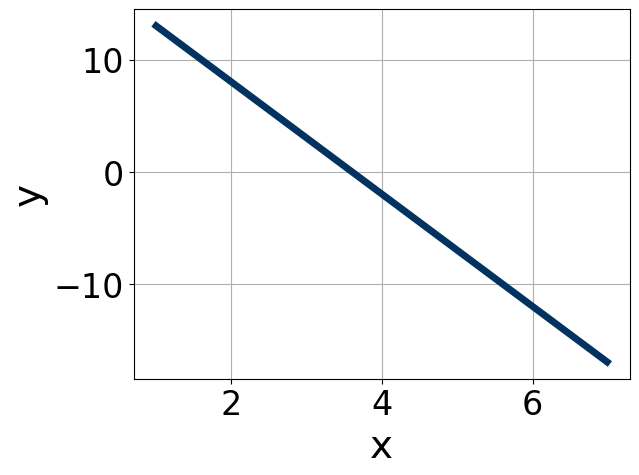
\includegraphics[width=0.5\textwidth]{../Figures/MA_8_F_1_2_graphB.png}
\end{center}


The solution is yes, the graph is linear., which is option A.

\begin{enumerate}[label=\Alph*.]
\item Yes, the graph is linear

* Correct! The graph has a constant rate of change and is thus a linear function.
\item No, the graph is not linear.

A linear function has a constant rate of growth. As $x$ increases/decreases, $y$ increases/decreases at the same rate. The graph in this example does have a constant rate of change.
\end{enumerate}


\textbf{General Comment:} The equation graphed was -5(x -4)-2. A linear function has a constant rate of growth. This means that as $x$ increases or decreases, $y$ increase or decreases at the same rate. For example, $x^2$ is NOT a linear function. As $x$ increases, the $y$ increases faster and faster. From $x=1$ to $x=2$, the $y$ increases by 3. From $x=2$ to $x=3$, the $y$ increases by 5. From $x=3$ to $x=4$, the $y$ increases by 7. A linear function would have the same change in $y$ for any change in $x$.
}
\litem{
Is the following relation a function?
\[ (-3, 135), (-2, 40), (-1, 5), (0, 0), (1, -5), (2, -40), (3, -135) \]The solution is Yes, which is option A.

\begin{enumerate}[label=\Alph*.]
\item Yes

* Correct! Every $x$-value has exactly one output.
\item No

For a relation to be a function, every $x$-value needs exactly one output. That means for a relation to NOT be a function, we would need one $x$-value that has two or more different outputs.
\end{enumerate}


\textbf{General Comment:} For a relation to be a function, every $x$-value needs exactly one output.
}
\litem{
Is the equation below a linear function?
\[ f(x) = {4}\sqrt{3x -7}+7 \]The solution is no, the equation is not linear., which is option B.

\begin{enumerate}[label=\Alph*.]
\item Yes, the equation is linear

A linear equation is a degree-1 polynomial. {4}\sqrt{3x -7}+7 is a square root function
\item No, the equation is not linear.

* Correct! {4}\sqrt{3x -7}+7 is not a degree-1 polynomial.
\end{enumerate}


\textbf{General Comment:} The equation graphed was {4}\sqrt{3x -7}+7. A linear function is a degree-1 polynomial. Polynomial equations have all variables with positive integer exponents, like $f(x) = 3x^2-2x+4$. Square root and cube root functions have rational exponents (1/2 and 1/3).
}
\litem{
Is the following relation a linear function?


\begin{tabular}{c|c}
x &y\tabularnewline \hline
1 &-3\tabularnewline \hline
2 &-12\tabularnewline \hline
3 &-27\tabularnewline \hline
4 &-48\tabularnewline \hline
5 &48\tabularnewline \hline
4 &3\tabularnewline \hline
3 &12\end{tabular}The solution is No, which is option B.

\begin{enumerate}[label=\Alph*.]
\item Yes

Notice how one $x$-value has two separate outputs? For a relation to be a function, every $x$-value needs exactly one output.
\item No

* Correct! An $x$-value has two separate outputs and thus this relation is not a function, let alone a linear function.
\end{enumerate}


\textbf{General Comment:} For a relation to be a linear function, every $x$-value needs exactly one output AND there needs to be a constant rate of growth (as $x$ increases/decreases, $y$ increases/decreases at the same rate).
}
\litem{
Is the graph below a linear function?

\begin{center}
    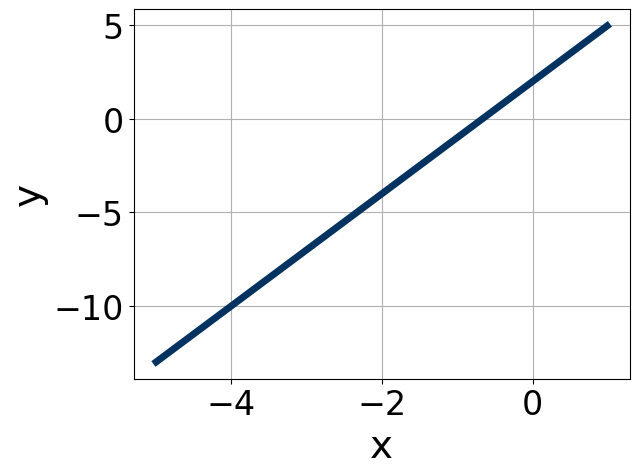
\includegraphics[width=0.5\textwidth]{../Figures/MA_8_F_1_2_graphC.png}
\end{center}


The solution is yes, the graph is linear., which is option A.

\begin{enumerate}[label=\Alph*.]
\item Yes, the graph is linear

* Correct! The graph has a constant rate of change and is thus a linear function.
\item No, the graph is not linear.

A linear function has a constant rate of growth. As $x$ increases/decreases, $y$ increases/decreases at the same rate. The graph in this example does have a constant rate of change.
\end{enumerate}


\textbf{General Comment:} The equation graphed was 3(x + 2)-4. A linear function has a constant rate of growth. This means that as $x$ increases or decreases, $y$ increase or decreases at the same rate. For example, $x^2$ is NOT a linear function. As $x$ increases, the $y$ increases faster and faster. From $x=1$ to $x=2$, the $y$ increases by 3. From $x=2$ to $x=3$, the $y$ increases by 5. From $x=3$ to $x=4$, the $y$ increases by 7. A linear function would have the same change in $y$ for any change in $x$.
}
\litem{
Is the following relation a function?


\begin{tabular}{c|c}
x &y\tabularnewline \hline
-1 &1\tabularnewline \hline
0 &0\tabularnewline \hline
1 &-1\tabularnewline \hline
2 &-8\tabularnewline \hline
3 &-27\tabularnewline \hline
4 &-64\tabularnewline \hline
5 &-125\end{tabular}The solution is Yes, which is option A.

\begin{enumerate}[label=\Alph*.]
\item Yes

* Correct! Every $x$-value has exactly one output.
\item No

For a relation to be a function, every $x$-value needs exactly one output. That means for a relation to NOT be a function, we would need one $x$-value that has two or more different outputs.
\end{enumerate}


\textbf{General Comment:} For a relation to be a function, every $x$-value needs exactly one output.
}
\litem{
Is the equation below a linear function?
\[ f(x) = 4 (2)^{x + 5}-3 \]The solution is no, the equation is not linear., which is option B.

\begin{enumerate}[label=\Alph*.]
\item Yes, the equation is linear

A linear equation is a degree-1 polynomial. 4 (2)^{x + 5}-3 is a base-2 exponential function
\item No, the equation is not linear.

* Correct! 4 (2)^{x + 5}-3 is not a degree-1 polynomial.
\end{enumerate}


\textbf{General Comment:} The equation graphed was 4 (2)^{x + 5}-3. A linear function is a degree-1 polynomial. Polynomial equations have all variables with positive integer exponents, like $f(x) = 3x^2-2x+4$. Square root and cube root functions have rational exponents (1/2 and 1/3).
}
\litem{
Is the following relation a linear function?


\begin{tabular}{c|c}
x &y\tabularnewline \hline
3 &-3.46\tabularnewline \hline
4 &-4.0\tabularnewline \hline
5 &-4.0\tabularnewline \hline
4 &3.46\tabularnewline \hline
3 &4.0\tabularnewline \hline
2 &4.47\tabularnewline \hline
1 &4.9\end{tabular}The solution is No, which is option B.

\begin{enumerate}[label=\Alph*.]
\item Yes

Notice how one $x$-value has two separate outputs? For a relation to be a function, every $x$-value needs exactly one output.
\item No

* Correct! An $x$-value has two separate outputs and thus this relation is not a function, let alone a linear function.
\end{enumerate}


\textbf{General Comment:} For a relation to be a linear function, every $x$-value needs exactly one output AND there needs to be a constant rate of growth (as $x$ increases/decreases, $y$ increases/decreases at the same rate).
}
\litem{
Is the graph below a linear function?

\begin{center}
    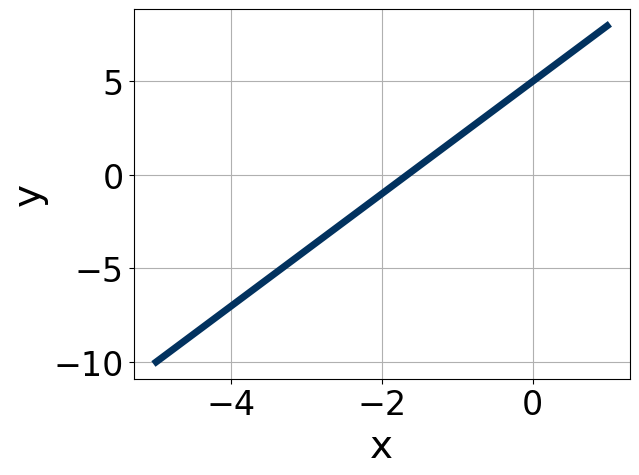
\includegraphics[width=0.5\textwidth]{../Figures/MA_8_F_1_2_graphD.png}
\end{center}


The solution is yes, the graph is linear., which is option A.

\begin{enumerate}[label=\Alph*.]
\item Yes, the graph is linear

* Correct! The graph has a constant rate of change and is thus a linear function.
\item No, the graph is not linear.

A linear function has a constant rate of growth. As $x$ increases/decreases, $y$ increases/decreases at the same rate. The graph in this example does have a constant rate of change.
\end{enumerate}


\textbf{General Comment:} The equation graphed was 3(x + 2)-1. A linear function has a constant rate of growth. This means that as $x$ increases or decreases, $y$ increase or decreases at the same rate. For example, $x^2$ is NOT a linear function. As $x$ increases, the $y$ increases faster and faster. From $x=1$ to $x=2$, the $y$ increases by 3. From $x=2$ to $x=3$, the $y$ increases by 5. From $x=3$ to $x=4$, the $y$ increases by 7. A linear function would have the same change in $y$ for any change in $x$.
}
\litem{
Is the following relation a function?
\[ (3, 0.12), (4, 0.06), (5, 0.03), (6, 0.02), (7, 0.01), (8, 0.0), (9, 0.0) \]The solution is Yes, which is option A.

\begin{enumerate}[label=\Alph*.]
\item Yes

* Correct! Every $x$-value has exactly one output.
\item No

For a relation to be a function, every $x$-value needs exactly one output. That means for a relation to NOT be a function, we would need one $x$-value that has two or more different outputs.
\end{enumerate}


\textbf{General Comment:} For a relation to be a function, every $x$-value needs exactly one output.
}
\litem{
Is the equation below a linear function?
\[ f(x) = -2(x -2)+2 \]The solution is yes, the graph is linear., which is option A.

\begin{enumerate}[label=\Alph*.]
\item Yes, the equation is linear

* Correct! The equation is a degree-1 polynomial and is thus a linear function.
\item No, the equation is not linear.

A linear function is a degree-1 polynomial. Polynomial equations have all variables with positive integer exponents.
\end{enumerate}


\textbf{General Comment:} The equation graphed was -2(x -2)+2. A linear function is a degree-1 polynomial. Polynomial equations have all variables with positive integer exponents, like $f(x) = 3x^2-2x+4$. Square root and cube root functions have rational exponents (1/2 and 1/3).
}
\litem{
Is the following relation a linear function?


\begin{tabular}{c|c}
x &y\tabularnewline \hline
3 &8.66\tabularnewline \hline
4 &10.0\tabularnewline \hline
5 &11.18\tabularnewline \hline
6 &-11.18\tabularnewline \hline
5 &-8.66\tabularnewline \hline
4 &-10.0\tabularnewline \hline
3 &-11.18\end{tabular}The solution is No, which is option B.

\begin{enumerate}[label=\Alph*.]
\item Yes

Notice how one $x$-value has two separate outputs? For a relation to be a function, every $x$-value needs exactly one output.
\item No

* Correct! An $x$-value has two separate outputs and thus this relation is not a function, let alone a linear function.
\end{enumerate}


\textbf{General Comment:} For a relation to be a linear function, every $x$-value needs exactly one output AND there needs to be a constant rate of growth (as $x$ increases/decreases, $y$ increases/decreases at the same rate).
}
\litem{
Is the graph below a linear function?

\begin{center}
    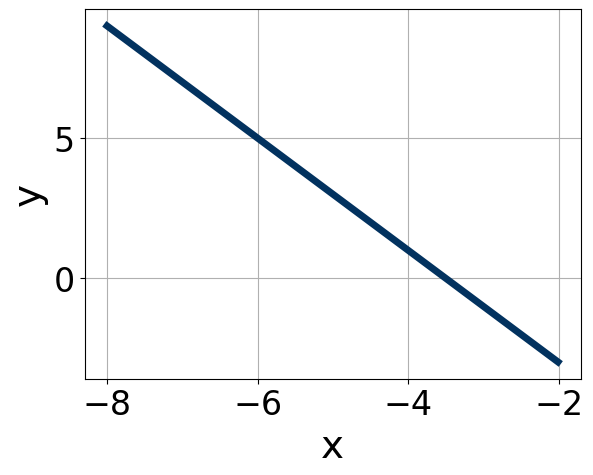
\includegraphics[width=0.5\textwidth]{../Figures/MA_8_F_1_2_graphE.png}
\end{center}


The solution is yes, the graph is linear., which is option A.

\begin{enumerate}[label=\Alph*.]
\item Yes, the graph is linear

* Correct! The graph has a constant rate of change and is thus a linear function.
\item No, the graph is not linear.

A linear function has a constant rate of growth. As $x$ increases/decreases, $y$ increases/decreases at the same rate. The graph in this example does have a constant rate of change.
\end{enumerate}


\textbf{General Comment:} The equation graphed was -2(x + 5)+3. A linear function has a constant rate of growth. This means that as $x$ increases or decreases, $y$ increase or decreases at the same rate. For example, $x^2$ is NOT a linear function. As $x$ increases, the $y$ increases faster and faster. From $x=1$ to $x=2$, the $y$ increases by 3. From $x=2$ to $x=3$, the $y$ increases by 5. From $x=3$ to $x=4$, the $y$ increases by 7. A linear function would have the same change in $y$ for any change in $x$.
}
\litem{
Is the following relation a function?


\begin{tabular}{c|c}
x &y\tabularnewline \hline
3 &-3\tabularnewline \hline
4 &-4\tabularnewline \hline
5 &-5\tabularnewline \hline
6 &-5\tabularnewline \hline
5 &3\tabularnewline \hline
4 &4\tabularnewline \hline
3 &5\end{tabular}The solution is No, which is option B.

\begin{enumerate}[label=\Alph*.]
\item Yes

Notice how one $x$-value has two separate outputs? For a relation to be a function, every $x$-value needs exactly one output.
\item No

* Correct! An $x$-value has two separate outputs and thus this relation is not a function.
\end{enumerate}


\textbf{General Comment:} For a relation to be a function, every $x$-value needs exactly one output.
}
\litem{
Is the equation below a linear function?
\[ f(x) = 2 \left( \dfrac{1}{2} \right)^{x -2}+1 \]The solution is no, the equation is not linear., which is option B.

\begin{enumerate}[label=\Alph*.]
\item Yes, the equation is linear

A linear equation is a degree-1 polynomial. 2 \left( \dfrac{1}{2} \right)^{x -2}+1 is a base-0.5 exponential function
\item No, the equation is not linear.

* Correct! 2 \left( \dfrac{1}{2} \right)^{x -2}+1 is not a degree-1 polynomial.
\end{enumerate}


\textbf{General Comment:} The equation graphed was 2 \left( \dfrac{1}{2} \right)^{x -2}+1. A linear function is a degree-1 polynomial. Polynomial equations have all variables with positive integer exponents, like $f(x) = 3x^2-2x+4$. Square root and cube root functions have rational exponents (1/2 and 1/3).
}
\litem{
Is the following relation a linear function?


\begin{tabular}{c|c}
x &y\tabularnewline \hline
2 &-7.07\tabularnewline \hline
3 &-8.66\tabularnewline \hline
4 &-8.66\tabularnewline \hline
3 &7.07\tabularnewline \hline
2 &8.66\tabularnewline \hline
1 &10.0\tabularnewline \hline
0 &11.18\end{tabular}The solution is No, which is option B.

\begin{enumerate}[label=\Alph*.]
\item Yes

Notice how one $x$-value has two separate outputs? For a relation to be a function, every $x$-value needs exactly one output.
\item No

* Correct! An $x$-value has two separate outputs and thus this relation is not a function, let alone a linear function.
\end{enumerate}


\textbf{General Comment:} For a relation to be a linear function, every $x$-value needs exactly one output AND there needs to be a constant rate of growth (as $x$ increases/decreases, $y$ increases/decreases at the same rate).
}
\litem{
Is the graph below a linear function?

\begin{center}
    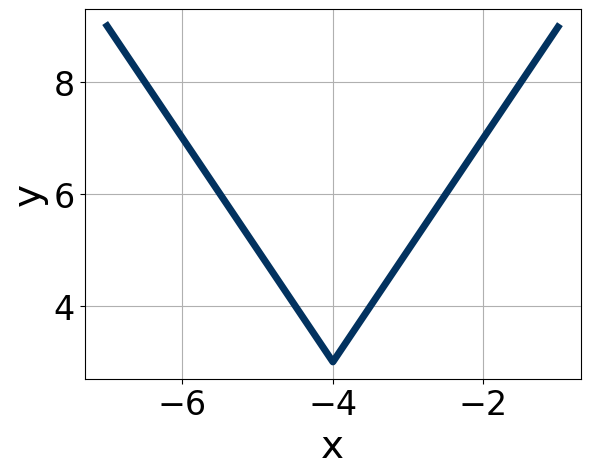
\includegraphics[width=0.5\textwidth]{../Figures/MA_8_F_1_2_graphF.png}
\end{center}


The solution is no, the graph is not linear., which is option B.

\begin{enumerate}[label=\Alph*.]
\item Yes, the graph is linear

A linear function has a constant rate of growth. As $x$ increases/decreases, $y$ increases/decreases at the same rate. The graph in this example does not have a constant rate of change.
\item No, the graph is not linear.

* Correct! The graph does not have a constant rate of change and thus is not a linear function.
\end{enumerate}


\textbf{General Comment:} The equation graphed was 2|x + 4|+3. A linear function has a constant rate of growth. This means that as $x$ increases or decreases, $y$ increase or decreases at the same rate. For example, $x^2$ is NOT a linear function. As $x$ increases, the $y$ increases faster and faster. From $x=1$ to $x=2$, the $y$ increases by 3. From $x=2$ to $x=3$, the $y$ increases by 5. From $x=3$ to $x=4$, the $y$ increases by 7. A linear function would have the same change in $y$ for any change in $x$.
}
\litem{
Is the following relation a function?


\begin{tabular}{c|c}
x &y\tabularnewline \hline
2 &-20\tabularnewline \hline
3 &-45\tabularnewline \hline
4 &-80\tabularnewline \hline
5 &-125\tabularnewline \hline
6 &125\tabularnewline \hline
5 &20\tabularnewline \hline
4 &45\end{tabular}The solution is No, which is option B.

\begin{enumerate}[label=\Alph*.]
\item Yes

Notice how one $x$-value has two separate outputs? For a relation to be a function, every $x$-value needs exactly one output.
\item No

* Correct! An $x$-value has two separate outputs and thus this relation is not a function.
\end{enumerate}


\textbf{General Comment:} For a relation to be a function, every $x$-value needs exactly one output.
}
\litem{
Is the equation below a linear function?
\[ f(x) = -2|x -1|+2 \]The solution is no, the equation is not linear., which is option B.

\begin{enumerate}[label=\Alph*.]
\item Yes, the equation is linear

A linear equation is a degree-1 polynomial. -2|x -1|+2 is a absolute value function
\item No, the equation is not linear.

* Correct! -2|x -1|+2 is not a degree-1 polynomial.
\end{enumerate}


\textbf{General Comment:} The equation graphed was -2|x -1|+2. A linear function is a degree-1 polynomial. Polynomial equations have all variables with positive integer exponents, like $f(x) = 3x^2-2x+4$. Square root and cube root functions have rational exponents (1/2 and 1/3).
}
\litem{
Is the following relation a linear function?


\begin{tabular}{c|c}
x &y\tabularnewline \hline
2 &-8\tabularnewline \hline
3 &-12\tabularnewline \hline
4 &-16\tabularnewline \hline
5 &16\tabularnewline \hline
4 &8\tabularnewline \hline
3 &12\tabularnewline \hline
2 &16\end{tabular}The solution is No, which is option B.

\begin{enumerate}[label=\Alph*.]
\item Yes

Notice how one $x$-value has two separate outputs? For a relation to be a function, every $x$-value needs exactly one output.
\item No

* Correct! An $x$-value has two separate outputs and thus this relation is not a function, let alone a linear function.
\end{enumerate}


\textbf{General Comment:} For a relation to be a linear function, every $x$-value needs exactly one output AND there needs to be a constant rate of growth (as $x$ increases/decreases, $y$ increases/decreases at the same rate).
}
\litem{
Is the graph below a linear function?

\begin{center}
    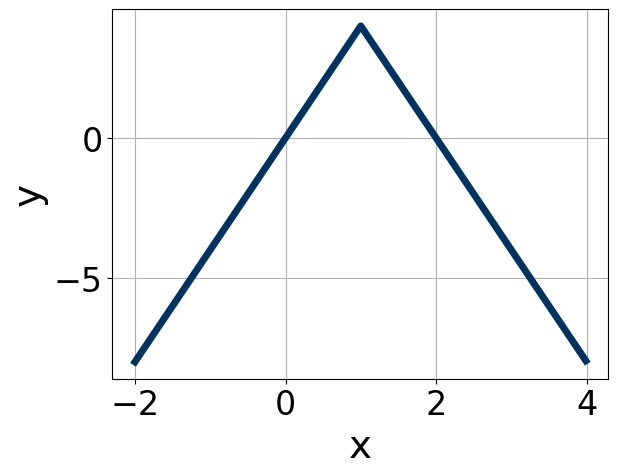
\includegraphics[width=0.5\textwidth]{../Figures/MA_8_F_1_2_graphG.png}
\end{center}


The solution is no, the graph is not linear., which is option B.

\begin{enumerate}[label=\Alph*.]
\item Yes, the graph is linear

A linear function has a constant rate of growth. As $x$ increases/decreases, $y$ increases/decreases at the same rate. The graph in this example does not have a constant rate of change.
\item No, the graph is not linear.

* Correct! The graph does not have a constant rate of change and thus is not a linear function.
\end{enumerate}


\textbf{General Comment:} The equation graphed was -4|x -1|+4. A linear function has a constant rate of growth. This means that as $x$ increases or decreases, $y$ increase or decreases at the same rate. For example, $x^2$ is NOT a linear function. As $x$ increases, the $y$ increases faster and faster. From $x=1$ to $x=2$, the $y$ increases by 3. From $x=2$ to $x=3$, the $y$ increases by 5. From $x=3$ to $x=4$, the $y$ increases by 7. A linear function would have the same change in $y$ for any change in $x$.
}
\litem{
Is the following relation a function?
\[ (4, 6.0), (5, 6.71), (6, 7.35), (7, 7.94), (8, -7.94), (7, -6.0), (6, -6.71) \]The solution is No, which is option B.

\begin{enumerate}[label=\Alph*.]
\item Yes

Notice how one $x$-value has two separate outputs? For a relation to be a function, every $x$-value needs exactly one output.
\item No

* Correct! An $x$-value has two separate outputs and thus this relation is not a function.
\end{enumerate}


\textbf{General Comment:} For a relation to be a function, every $x$-value needs exactly one output.
}
\litem{
Is the equation below a linear function?
\[ f(x) = {-3}\sqrt{4x + 5}+6 \]The solution is no, the equation is not linear., which is option B.

\begin{enumerate}[label=\Alph*.]
\item Yes, the equation is linear

A linear equation is a degree-1 polynomial. {-3}\sqrt{4x + 5}+6 is a square root function
\item No, the equation is not linear.

* Correct! {-3}\sqrt{4x + 5}+6 is not a degree-1 polynomial.
\end{enumerate}


\textbf{General Comment:} The equation graphed was {-3}\sqrt{4x + 5}+6. A linear function is a degree-1 polynomial. Polynomial equations have all variables with positive integer exponents, like $f(x) = 3x^2-2x+4$. Square root and cube root functions have rational exponents (1/2 and 1/3).
}
\litem{
Is the following relation a linear function?


\begin{tabular}{c|c}
x &y\tabularnewline \hline
-2 &-5\tabularnewline \hline
-1 &-2\tabularnewline \hline
0 &1\tabularnewline \hline
1 &4\tabularnewline \hline
2 &7\tabularnewline \hline
3 &10\tabularnewline \hline
4 &13\end{tabular}The solution is Yes, which is option A.

\begin{enumerate}[label=\Alph*.]
\item Yes

* Correct! As $x$ increases/decreases, $y$ increases/decreases at the same rate.
\item No

A linear function has a constant rate of growth. As $x$ increases/decreases, $y$ increases/decreases at the same rate.
\end{enumerate}


\textbf{General Comment:} For a relation to be a linear function, every $x$-value needs exactly one output AND there needs to be a constant rate of growth (as $x$ increases/decreases, $y$ increases/decreases at the same rate).
}
\litem{
Is the graph below a linear function?

\begin{center}
    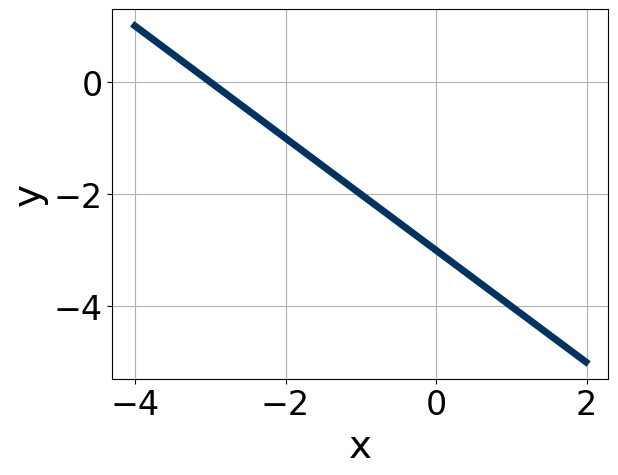
\includegraphics[width=0.5\textwidth]{../Figures/MA_8_F_1_2_graphH.png}
\end{center}


The solution is yes, the graph is linear., which is option A.

\begin{enumerate}[label=\Alph*.]
\item Yes, the graph is linear

* Correct! The graph has a constant rate of change and is thus a linear function.
\item No, the graph is not linear.

A linear function has a constant rate of growth. As $x$ increases/decreases, $y$ increases/decreases at the same rate. The graph in this example does have a constant rate of change.
\end{enumerate}


\textbf{General Comment:} The equation graphed was -1(x + 1)-2. A linear function has a constant rate of growth. This means that as $x$ increases or decreases, $y$ increase or decreases at the same rate. For example, $x^2$ is NOT a linear function. As $x$ increases, the $y$ increases faster and faster. From $x=1$ to $x=2$, the $y$ increases by 3. From $x=2$ to $x=3$, the $y$ increases by 5. From $x=3$ to $x=4$, the $y$ increases by 7. A linear function would have the same change in $y$ for any change in $x$.
}
\litem{
Is the following relation a function?


\begin{tabular}{c|c}
x &y\tabularnewline \hline
1 &-5\tabularnewline \hline
2 &-10\tabularnewline \hline
3 &-15\tabularnewline \hline
4 &-20\tabularnewline \hline
5 &20\tabularnewline \hline
4 &5\tabularnewline \hline
3 &10\end{tabular}The solution is No, which is option B.

\begin{enumerate}[label=\Alph*.]
\item Yes

Notice how one $x$-value has two separate outputs? For a relation to be a function, every $x$-value needs exactly one output.
\item No

* Correct! An $x$-value has two separate outputs and thus this relation is not a function.
\end{enumerate}


\textbf{General Comment:} For a relation to be a function, every $x$-value needs exactly one output.
}
\litem{
Is the equation below a linear function?
\[ f(x) = -2|x -3|+2 \]The solution is no, the equation is not linear., which is option B.

\begin{enumerate}[label=\Alph*.]
\item Yes, the equation is linear

A linear equation is a degree-1 polynomial. -2|x -3|+2 is a absolute value function
\item No, the equation is not linear.

* Correct! -2|x -3|+2 is not a degree-1 polynomial.
\end{enumerate}


\textbf{General Comment:} The equation graphed was -2|x -3|+2. A linear function is a degree-1 polynomial. Polynomial equations have all variables with positive integer exponents, like $f(x) = 3x^2-2x+4$. Square root and cube root functions have rational exponents (1/2 and 1/3).
}
\litem{
Is the following relation a linear function?


\begin{tabular}{c|c}
x &y\tabularnewline \hline
-3 &-14\tabularnewline \hline
-2 &-7\tabularnewline \hline
-1 &0\tabularnewline \hline
0 &7\tabularnewline \hline
1 &14\tabularnewline \hline
2 &21\tabularnewline \hline
3 &28\end{tabular}The solution is Yes, which is option A.

\begin{enumerate}[label=\Alph*.]
\item Yes

* Correct! As $x$ increases/decreases, $y$ increases/decreases at the same rate.
\item No

A linear function has a constant rate of growth. As $x$ increases/decreases, $y$ increases/decreases at the same rate.
\end{enumerate}


\textbf{General Comment:} For a relation to be a linear function, every $x$-value needs exactly one output AND there needs to be a constant rate of growth (as $x$ increases/decreases, $y$ increases/decreases at the same rate).
}
\litem{
Is the graph below a linear function?

\begin{center}
    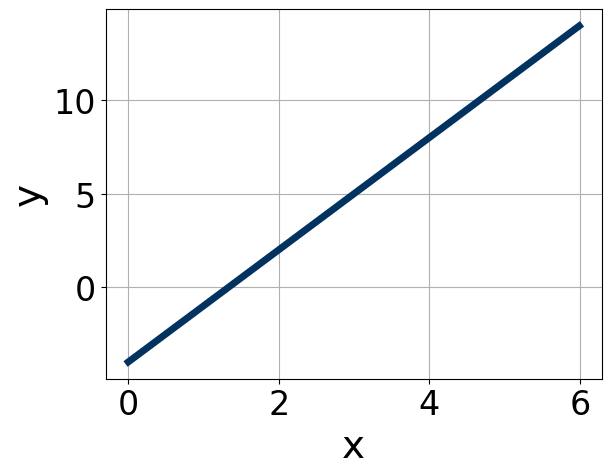
\includegraphics[width=0.5\textwidth]{../Figures/MA_8_F_1_2_graphI.png}
\end{center}


The solution is yes, the graph is linear., which is option A.

\begin{enumerate}[label=\Alph*.]
\item Yes, the graph is linear

* Correct! The graph has a constant rate of change and is thus a linear function.
\item No, the graph is not linear.

A linear function has a constant rate of growth. As $x$ increases/decreases, $y$ increases/decreases at the same rate. The graph in this example does have a constant rate of change.
\end{enumerate}


\textbf{General Comment:} The equation graphed was 3(x -3)+5. A linear function has a constant rate of growth. This means that as $x$ increases or decreases, $y$ increase or decreases at the same rate. For example, $x^2$ is NOT a linear function. As $x$ increases, the $y$ increases faster and faster. From $x=1$ to $x=2$, the $y$ increases by 3. From $x=2$ to $x=3$, the $y$ increases by 5. From $x=3$ to $x=4$, the $y$ increases by 7. A linear function would have the same change in $y$ for any change in $x$.
}
\litem{
Is the following relation a function?


\begin{tabular}{c|c}
x &y\tabularnewline \hline
2 &1.41\tabularnewline \hline
3 &1.73\tabularnewline \hline
4 &2.0\tabularnewline \hline
5 &-2.0\tabularnewline \hline
4 &-1.41\tabularnewline \hline
3 &-1.73\tabularnewline \hline
2 &-2.0\end{tabular}The solution is No, which is option B.

\begin{enumerate}[label=\Alph*.]
\item Yes

Notice how one $x$-value has two separate outputs? For a relation to be a function, every $x$-value needs exactly one output.
\item No

* Correct! An $x$-value has two separate outputs and thus this relation is not a function.
\end{enumerate}


\textbf{General Comment:} For a relation to be a function, every $x$-value needs exactly one output.
}
\litem{
Is the equation below a linear function?
\[ f(x) = 5(x -1)-5 \]The solution is yes, the graph is linear., which is option A.

\begin{enumerate}[label=\Alph*.]
\item Yes, the equation is linear

* Correct! The equation is a degree-1 polynomial and is thus a linear function.
\item No, the equation is not linear.

A linear function is a degree-1 polynomial. Polynomial equations have all variables with positive integer exponents.
\end{enumerate}


\textbf{General Comment:} The equation graphed was 5(x -1)-5. A linear function is a degree-1 polynomial. Polynomial equations have all variables with positive integer exponents, like $f(x) = 3x^2-2x+4$. Square root and cube root functions have rational exponents (1/2 and 1/3).
}
\litem{
Is the following relation a linear function?


\begin{tabular}{c|c}
x &y\tabularnewline \hline
3 &-9\tabularnewline \hline
4 &-16\tabularnewline \hline
5 &-25\tabularnewline \hline
6 &-25\tabularnewline \hline
5 &9\tabularnewline \hline
4 &16\tabularnewline \hline
3 &25\end{tabular}The solution is No, which is option B.

\begin{enumerate}[label=\Alph*.]
\item Yes

Notice how one $x$-value has two separate outputs? For a relation to be a function, every $x$-value needs exactly one output.
\item No

* Correct! An $x$-value has two separate outputs and thus this relation is not a function, let alone a linear function.
\end{enumerate}


\textbf{General Comment:} For a relation to be a linear function, every $x$-value needs exactly one output AND there needs to be a constant rate of growth (as $x$ increases/decreases, $y$ increases/decreases at the same rate).
}
\litem{
Is the graph below a linear function?

\begin{center}
    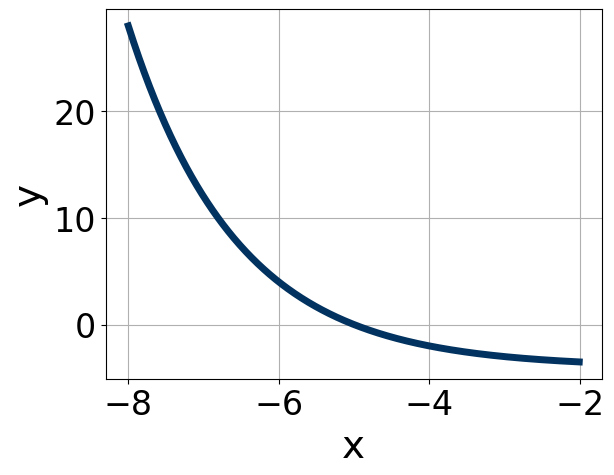
\includegraphics[width=0.5\textwidth]{../Figures/MA_8_F_1_2_graphJ.png}
\end{center}


The solution is no, the graph is not linear., which is option B.

\begin{enumerate}[label=\Alph*.]
\item Yes, the graph is linear

A linear function has a constant rate of growth. As $x$ increases/decreases, $y$ increases/decreases at the same rate. The graph in this example does not have a constant rate of change.
\item No, the graph is not linear.

* Correct! The graph does not have a constant rate of change and thus is not a linear function.
\end{enumerate}


\textbf{General Comment:} The equation graphed was 4 \left( \dfrac{1}{2} \right)^{x--5}-4. A linear function has a constant rate of growth. This means that as $x$ increases or decreases, $y$ increase or decreases at the same rate. For example, $x^2$ is NOT a linear function. As $x$ increases, the $y$ increases faster and faster. From $x=1$ to $x=2$, the $y$ increases by 3. From $x=2$ to $x=3$, the $y$ increases by 5. From $x=3$ to $x=4$, the $y$ increases by 7. A linear function would have the same change in $y$ for any change in $x$.
}
\litem{
Is the following relation a function?


\begin{tabular}{c|c}
x &y\tabularnewline \hline
2 &8\tabularnewline \hline
3 &12\tabularnewline \hline
4 &16\tabularnewline \hline
5 &16\tabularnewline \hline
4 &-8\tabularnewline \hline
3 &-12\tabularnewline \hline
2 &-16\end{tabular}The solution is No, which is option B.

\begin{enumerate}[label=\Alph*.]
\item Yes

Notice how one $x$-value has two separate outputs? For a relation to be a function, every $x$-value needs exactly one output.
\item No

* Correct! An $x$-value has two separate outputs and thus this relation is not a function.
\end{enumerate}


\textbf{General Comment:} For a relation to be a function, every $x$-value needs exactly one output.
}
\litem{
Is the equation below a linear function?
\[ f(x) = 2(x -3)-1 \]The solution is yes, the graph is linear., which is option A.

\begin{enumerate}[label=\Alph*.]
\item Yes, the equation is linear

* Correct! The equation is a degree-1 polynomial and is thus a linear function.
\item No, the equation is not linear.

A linear function is a degree-1 polynomial. Polynomial equations have all variables with positive integer exponents.
\end{enumerate}


\textbf{General Comment:} The equation graphed was 2(x -3)-1. A linear function is a degree-1 polynomial. Polynomial equations have all variables with positive integer exponents, like $f(x) = 3x^2-2x+4$. Square root and cube root functions have rational exponents (1/2 and 1/3).
}
\litem{
Is the following relation a linear function?


\begin{tabular}{c|c}
x &y\tabularnewline \hline
1 &-3.0\tabularnewline \hline
2 &-4.24\tabularnewline \hline
3 &4.24\tabularnewline \hline
2 &3.0\tabularnewline \hline
1 &4.24\tabularnewline \hline
0 &5.2\tabularnewline \hline
-1 &6.0\end{tabular}The solution is No, which is option B.

\begin{enumerate}[label=\Alph*.]
\item Yes

Notice how one $x$-value has two separate outputs? For a relation to be a function, every $x$-value needs exactly one output.
\item No

* Correct! An $x$-value has two separate outputs and thus this relation is not a function, let alone a linear function.
\end{enumerate}


\textbf{General Comment:} For a relation to be a linear function, every $x$-value needs exactly one output AND there needs to be a constant rate of growth (as $x$ increases/decreases, $y$ increases/decreases at the same rate).
}
\litem{
Is the graph below a linear function?

\begin{center}
    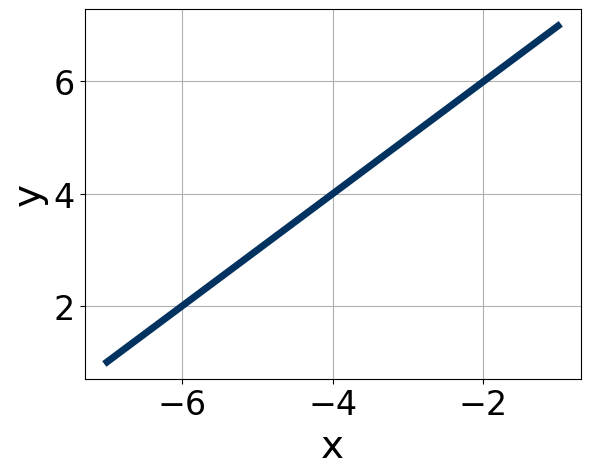
\includegraphics[width=0.5\textwidth]{../Figures/MA_8_F_1_2_graphK.png}
\end{center}


The solution is yes, the graph is linear., which is option A.

\begin{enumerate}[label=\Alph*.]
\item Yes, the graph is linear

* Correct! The graph has a constant rate of change and is thus a linear function.
\item No, the graph is not linear.

A linear function has a constant rate of growth. As $x$ increases/decreases, $y$ increases/decreases at the same rate. The graph in this example does have a constant rate of change.
\end{enumerate}


\textbf{General Comment:} The equation graphed was 1(x + 4)+4. A linear function has a constant rate of growth. This means that as $x$ increases or decreases, $y$ increase or decreases at the same rate. For example, $x^2$ is NOT a linear function. As $x$ increases, the $y$ increases faster and faster. From $x=1$ to $x=2$, the $y$ increases by 3. From $x=2$ to $x=3$, the $y$ increases by 5. From $x=3$ to $x=4$, the $y$ increases by 7. A linear function would have the same change in $y$ for any change in $x$.
}
\litem{
Is the following relation a function?
\[ (1, -4.0), (2, -5.66), (3, -6.93), (4, -8.0), (5, -8.94), (6, -9.8), (7, -10.58) \]The solution is Yes, which is option A.

\begin{enumerate}[label=\Alph*.]
\item Yes

* Correct! Every $x$-value has exactly one output.
\item No

For a relation to be a function, every $x$-value needs exactly one output. That means for a relation to NOT be a function, we would need one $x$-value that has two or more different outputs.
\end{enumerate}


\textbf{General Comment:} For a relation to be a function, every $x$-value needs exactly one output.
}
\litem{
Is the equation below a linear function?
\[ f(x) = 5(x + 5)-3 \]The solution is yes, the graph is linear., which is option A.

\begin{enumerate}[label=\Alph*.]
\item Yes, the equation is linear

* Correct! The equation is a degree-1 polynomial and is thus a linear function.
\item No, the equation is not linear.

A linear function is a degree-1 polynomial. Polynomial equations have all variables with positive integer exponents.
\end{enumerate}


\textbf{General Comment:} The equation graphed was 5(x + 5)-3. A linear function is a degree-1 polynomial. Polynomial equations have all variables with positive integer exponents, like $f(x) = 3x^2-2x+4$. Square root and cube root functions have rational exponents (1/2 and 1/3).
}
\litem{
Is the following relation a linear function?


\begin{tabular}{c|c}
x &y\tabularnewline \hline
1 &4.0\tabularnewline \hline
2 &5.66\tabularnewline \hline
3 &6.93\tabularnewline \hline
4 &8.0\tabularnewline \hline
5 &8.94\tabularnewline \hline
6 &9.8\tabularnewline \hline
7 &10.58\end{tabular}The solution is No, which is option B.

\begin{enumerate}[label=\Alph*.]
\item Yes

A linear function has a constant rate of growth. As $x$ increases/decreases, $y$ increases/decreases at the same rate. The table in this example does have a constant rate of change.
\item No

* Correct! The table in this example does not have a constant rate of change. This relation is a float function.
\end{enumerate}


\textbf{General Comment:} For a relation to be a linear function, every $x$-value needs exactly one output AND there needs to be a constant rate of growth (as $x$ increases/decreases, $y$ increases/decreases at the same rate).
}
\litem{
Is the graph below a linear function?

\begin{center}
    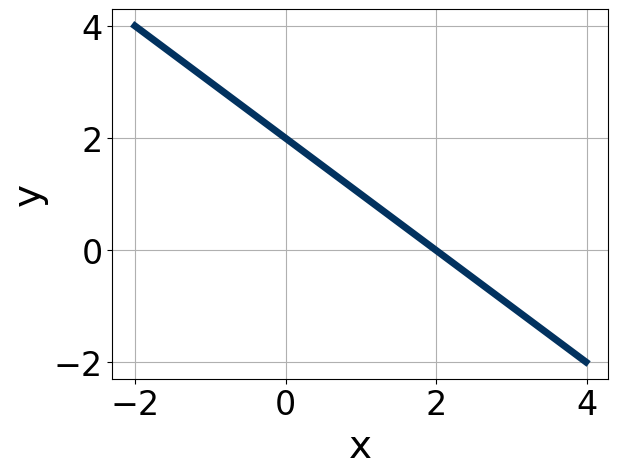
\includegraphics[width=0.5\textwidth]{../Figures/MA_8_F_1_2_graphL.png}
\end{center}


The solution is yes, the graph is linear., which is option A.

\begin{enumerate}[label=\Alph*.]
\item Yes, the graph is linear

* Correct! The graph has a constant rate of change and is thus a linear function.
\item No, the graph is not linear.

A linear function has a constant rate of growth. As $x$ increases/decreases, $y$ increases/decreases at the same rate. The graph in this example does have a constant rate of change.
\end{enumerate}


\textbf{General Comment:} The equation graphed was -1(x -1)+1. A linear function has a constant rate of growth. This means that as $x$ increases or decreases, $y$ increase or decreases at the same rate. For example, $x^2$ is NOT a linear function. As $x$ increases, the $y$ increases faster and faster. From $x=1$ to $x=2$, the $y$ increases by 3. From $x=2$ to $x=3$, the $y$ increases by 5. From $x=3$ to $x=4$, the $y$ increases by 7. A linear function would have the same change in $y$ for any change in $x$.
}
\litem{
Is the following relation a function?


\begin{tabular}{c|c}
x &y\tabularnewline \hline
2 &-16\tabularnewline \hline
3 &-54\tabularnewline \hline
4 &-128\tabularnewline \hline
5 &-250\tabularnewline \hline
6 &-432\tabularnewline \hline
7 &-686\tabularnewline \hline
8 &-1024\end{tabular}The solution is Yes, which is option A.

\begin{enumerate}[label=\Alph*.]
\item Yes

* Correct! Every $x$-value has exactly one output.
\item No

For a relation to be a function, every $x$-value needs exactly one output. That means for a relation to NOT be a function, we would need one $x$-value that has two or more different outputs.
\end{enumerate}


\textbf{General Comment:} For a relation to be a function, every $x$-value needs exactly one output.
}
\litem{
Is the equation below a linear function?
\[ f(x) = 3(x + 5)-5 \]The solution is yes, the graph is linear., which is option A.

\begin{enumerate}[label=\Alph*.]
\item Yes, the equation is linear

* Correct! The equation is a degree-1 polynomial and is thus a linear function.
\item No, the equation is not linear.

A linear function is a degree-1 polynomial. Polynomial equations have all variables with positive integer exponents.
\end{enumerate}


\textbf{General Comment:} The equation graphed was 3(x + 5)-5. A linear function is a degree-1 polynomial. Polynomial equations have all variables with positive integer exponents, like $f(x) = 3x^2-2x+4$. Square root and cube root functions have rational exponents (1/2 and 1/3).
}
\litem{
Is the following relation a linear function?


\begin{tabular}{c|c}
x &y\tabularnewline \hline
1 &2.0\tabularnewline \hline
2 &2.83\tabularnewline \hline
3 &3.46\tabularnewline \hline
4 &4.0\tabularnewline \hline
5 &4.47\tabularnewline \hline
6 &4.9\tabularnewline \hline
7 &5.29\end{tabular}The solution is No, which is option B.

\begin{enumerate}[label=\Alph*.]
\item Yes

A linear function has a constant rate of growth. As $x$ increases/decreases, $y$ increases/decreases at the same rate. The table in this example does have a constant rate of change.
\item No

* Correct! The table in this example does not have a constant rate of change. This relation is a float function.
\end{enumerate}


\textbf{General Comment:} For a relation to be a linear function, every $x$-value needs exactly one output AND there needs to be a constant rate of growth (as $x$ increases/decreases, $y$ increases/decreases at the same rate).
}
\litem{
Is the graph below a linear function?

\begin{center}
    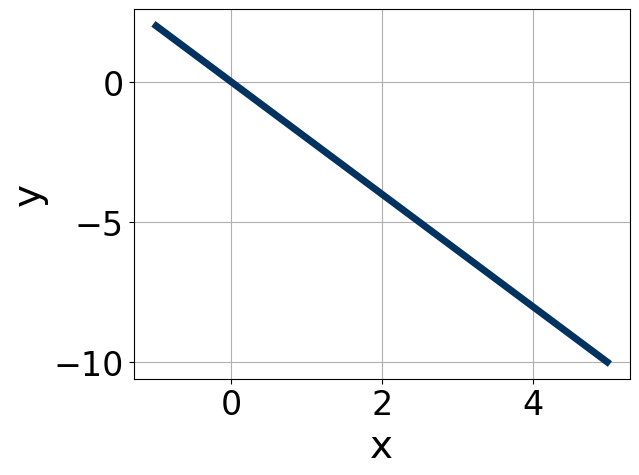
\includegraphics[width=0.5\textwidth]{../Figures/MA_8_F_1_2_graphM.png}
\end{center}


The solution is yes, the graph is linear., which is option A.

\begin{enumerate}[label=\Alph*.]
\item Yes, the graph is linear

* Correct! The graph has a constant rate of change and is thus a linear function.
\item No, the graph is not linear.

A linear function has a constant rate of growth. As $x$ increases/decreases, $y$ increases/decreases at the same rate. The graph in this example does have a constant rate of change.
\end{enumerate}


\textbf{General Comment:} The equation graphed was -2(x -2)-4. A linear function has a constant rate of growth. This means that as $x$ increases or decreases, $y$ increase or decreases at the same rate. For example, $x^2$ is NOT a linear function. As $x$ increases, the $y$ increases faster and faster. From $x=1$ to $x=2$, the $y$ increases by 3. From $x=2$ to $x=3$, the $y$ increases by 5. From $x=3$ to $x=4$, the $y$ increases by 7. A linear function would have the same change in $y$ for any change in $x$.
}
\litem{
Is the following relation a function?


\begin{tabular}{c|c}
x &y\tabularnewline \hline
4 &-64\tabularnewline \hline
5 &-125\tabularnewline \hline
6 &-216\tabularnewline \hline
7 &-343\tabularnewline \hline
8 &-512\tabularnewline \hline
9 &-729\tabularnewline \hline
10 &-1000\end{tabular}The solution is Yes, which is option A.

\begin{enumerate}[label=\Alph*.]
\item Yes

* Correct! Every $x$-value has exactly one output.
\item No

For a relation to be a function, every $x$-value needs exactly one output. That means for a relation to NOT be a function, we would need one $x$-value that has two or more different outputs.
\end{enumerate}


\textbf{General Comment:} For a relation to be a function, every $x$-value needs exactly one output.
}
\litem{
Is the equation below a linear function?
\[ f(x) = {-3}\sqrt[3]{-6x + 7}+4 \]The solution is no, the equation is not linear., which is option B.

\begin{enumerate}[label=\Alph*.]
\item Yes, the equation is linear

A linear equation is a degree-1 polynomial. {-3}\sqrt[3]{-6x + 7}+4 is a cube root function
\item No, the equation is not linear.

* Correct! {-3}\sqrt[3]{-6x + 7}+4 is not a degree-1 polynomial.
\end{enumerate}


\textbf{General Comment:} The equation graphed was {-3}\sqrt[3]{-6x + 7}+4. A linear function is a degree-1 polynomial. Polynomial equations have all variables with positive integer exponents, like $f(x) = 3x^2-2x+4$. Square root and cube root functions have rational exponents (1/2 and 1/3).
}
\litem{
Is the following relation a linear function?


\begin{tabular}{c|c}
x &y\tabularnewline \hline
1 &1.0\tabularnewline \hline
2 &1.41\tabularnewline \hline
3 &1.73\tabularnewline \hline
4 &-1.73\tabularnewline \hline
3 &-1.0\tabularnewline \hline
2 &-1.41\tabularnewline \hline
1 &-1.73\end{tabular}The solution is No, which is option B.

\begin{enumerate}[label=\Alph*.]
\item Yes

Notice how one $x$-value has two separate outputs? For a relation to be a function, every $x$-value needs exactly one output.
\item No

* Correct! An $x$-value has two separate outputs and thus this relation is not a function, let alone a linear function.
\end{enumerate}


\textbf{General Comment:} For a relation to be a linear function, every $x$-value needs exactly one output AND there needs to be a constant rate of growth (as $x$ increases/decreases, $y$ increases/decreases at the same rate).
}
\litem{
Is the graph below a linear function?

\begin{center}
    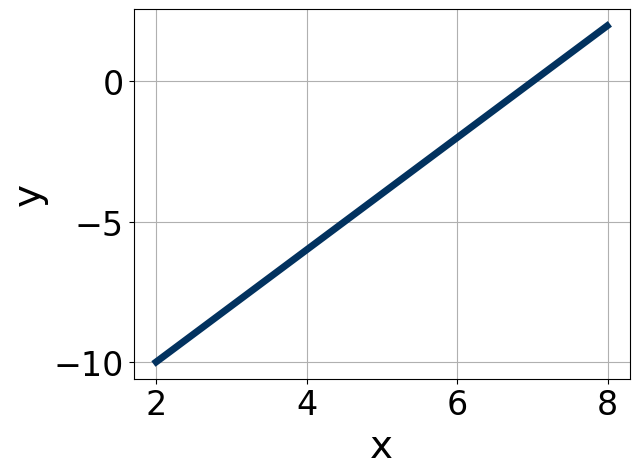
\includegraphics[width=0.5\textwidth]{../Figures/MA_8_F_1_2_graphN.png}
\end{center}


The solution is yes, the graph is linear., which is option A.

\begin{enumerate}[label=\Alph*.]
\item Yes, the graph is linear

* Correct! The graph has a constant rate of change and is thus a linear function.
\item No, the graph is not linear.

A linear function has a constant rate of growth. As $x$ increases/decreases, $y$ increases/decreases at the same rate. The graph in this example does have a constant rate of change.
\end{enumerate}


\textbf{General Comment:} The equation graphed was 2(x -5)-4. A linear function has a constant rate of growth. This means that as $x$ increases or decreases, $y$ increase or decreases at the same rate. For example, $x^2$ is NOT a linear function. As $x$ increases, the $y$ increases faster and faster. From $x=1$ to $x=2$, the $y$ increases by 3. From $x=2$ to $x=3$, the $y$ increases by 5. From $x=3$ to $x=4$, the $y$ increases by 7. A linear function would have the same change in $y$ for any change in $x$.
}
\litem{
Is the following relation a function?


\begin{tabular}{c|c}
x &y\tabularnewline \hline
1 &5.0\tabularnewline \hline
2 &7.07\tabularnewline \hline
3 &8.66\tabularnewline \hline
4 &10.0\tabularnewline \hline
5 &-10.0\tabularnewline \hline
4 &-5.0\tabularnewline \hline
3 &-7.07\end{tabular}The solution is No, which is option B.

\begin{enumerate}[label=\Alph*.]
\item Yes

Notice how one $x$-value has two separate outputs? For a relation to be a function, every $x$-value needs exactly one output.
\item No

* Correct! An $x$-value has two separate outputs and thus this relation is not a function.
\end{enumerate}


\textbf{General Comment:} For a relation to be a function, every $x$-value needs exactly one output.
}
\litem{
Is the equation below a linear function?
\[ f(x) = 4(x + 4)+1 \]The solution is yes, the graph is linear., which is option A.

\begin{enumerate}[label=\Alph*.]
\item Yes, the equation is linear

* Correct! The equation is a degree-1 polynomial and is thus a linear function.
\item No, the equation is not linear.

A linear function is a degree-1 polynomial. Polynomial equations have all variables with positive integer exponents.
\end{enumerate}


\textbf{General Comment:} The equation graphed was 4(x + 4)+1. A linear function is a degree-1 polynomial. Polynomial equations have all variables with positive integer exponents, like $f(x) = 3x^2-2x+4$. Square root and cube root functions have rational exponents (1/2 and 1/3).
}
\litem{
Is the following relation a linear function?


\begin{tabular}{c|c}
x &y\tabularnewline \hline
4 &10.0\tabularnewline \hline
5 &11.18\tabularnewline \hline
6 &12.25\tabularnewline \hline
7 &-12.25\tabularnewline \hline
6 &-10.0\tabularnewline \hline
5 &-11.18\tabularnewline \hline
4 &-12.25\end{tabular}The solution is No, which is option B.

\begin{enumerate}[label=\Alph*.]
\item Yes

Notice how one $x$-value has two separate outputs? For a relation to be a function, every $x$-value needs exactly one output.
\item No

* Correct! An $x$-value has two separate outputs and thus this relation is not a function, let alone a linear function.
\end{enumerate}


\textbf{General Comment:} For a relation to be a linear function, every $x$-value needs exactly one output AND there needs to be a constant rate of growth (as $x$ increases/decreases, $y$ increases/decreases at the same rate).
}
\litem{
Is the graph below a linear function?

\begin{center}
    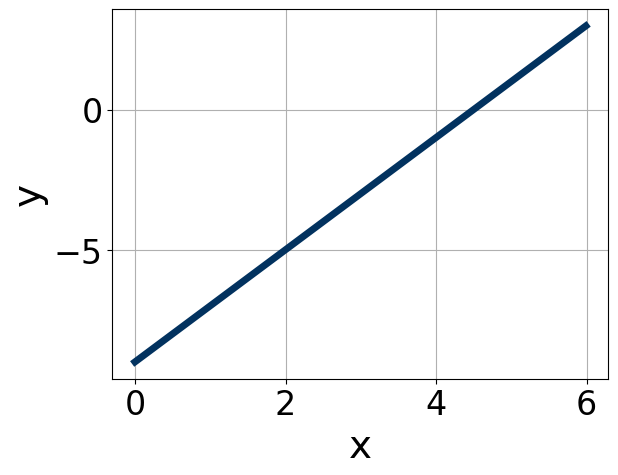
\includegraphics[width=0.5\textwidth]{../Figures/MA_8_F_1_2_graphO.png}
\end{center}


The solution is yes, the graph is linear., which is option A.

\begin{enumerate}[label=\Alph*.]
\item Yes, the graph is linear

* Correct! The graph has a constant rate of change and is thus a linear function.
\item No, the graph is not linear.

A linear function has a constant rate of growth. As $x$ increases/decreases, $y$ increases/decreases at the same rate. The graph in this example does have a constant rate of change.
\end{enumerate}


\textbf{General Comment:} The equation graphed was 2(x -3)-3. A linear function has a constant rate of growth. This means that as $x$ increases or decreases, $y$ increase or decreases at the same rate. For example, $x^2$ is NOT a linear function. As $x$ increases, the $y$ increases faster and faster. From $x=1$ to $x=2$, the $y$ increases by 3. From $x=2$ to $x=3$, the $y$ increases by 5. From $x=3$ to $x=4$, the $y$ increases by 7. A linear function would have the same change in $y$ for any change in $x$.
}
\litem{
Is the following relation a function?


\begin{tabular}{c|c}
x &y\tabularnewline \hline
1 &10\tabularnewline \hline
2 &14\tabularnewline \hline
3 &18\tabularnewline \hline
4 &22\tabularnewline \hline
5 &26\tabularnewline \hline
6 &30\tabularnewline \hline
7 &34\end{tabular}The solution is Yes, which is option A.

\begin{enumerate}[label=\Alph*.]
\item Yes

* Correct! Every $x$-value has exactly one output.
\item No

For a relation to be a function, every $x$-value needs exactly one output. That means for a relation to NOT be a function, we would need one $x$-value that has two or more different outputs.
\end{enumerate}


\textbf{General Comment:} For a relation to be a function, every $x$-value needs exactly one output.
}
\litem{
Is the equation below a linear function?
\[ f(x) = 3(x -5)-4 \]The solution is yes, the graph is linear., which is option A.

\begin{enumerate}[label=\Alph*.]
\item Yes, the equation is linear

* Correct! The equation is a degree-1 polynomial and is thus a linear function.
\item No, the equation is not linear.

A linear function is a degree-1 polynomial. Polynomial equations have all variables with positive integer exponents.
\end{enumerate}


\textbf{General Comment:} The equation graphed was 3(x -5)-4. A linear function is a degree-1 polynomial. Polynomial equations have all variables with positive integer exponents, like $f(x) = 3x^2-2x+4$. Square root and cube root functions have rational exponents (1/2 and 1/3).
}
\litem{
Is the following relation a linear function?


\begin{tabular}{c|c}
x &y\tabularnewline \hline
1 &-5\tabularnewline \hline
2 &-20\tabularnewline \hline
3 &-45\tabularnewline \hline
4 &-80\tabularnewline \hline
5 &-80\tabularnewline \hline
4 &5\tabularnewline \hline
3 &20\end{tabular}The solution is No, which is option B.

\begin{enumerate}[label=\Alph*.]
\item Yes

Notice how one $x$-value has two separate outputs? For a relation to be a function, every $x$-value needs exactly one output.
\item No

* Correct! An $x$-value has two separate outputs and thus this relation is not a function, let alone a linear function.
\end{enumerate}


\textbf{General Comment:} For a relation to be a linear function, every $x$-value needs exactly one output AND there needs to be a constant rate of growth (as $x$ increases/decreases, $y$ increases/decreases at the same rate).
}
\litem{
Is the graph below a linear function?

\begin{center}
    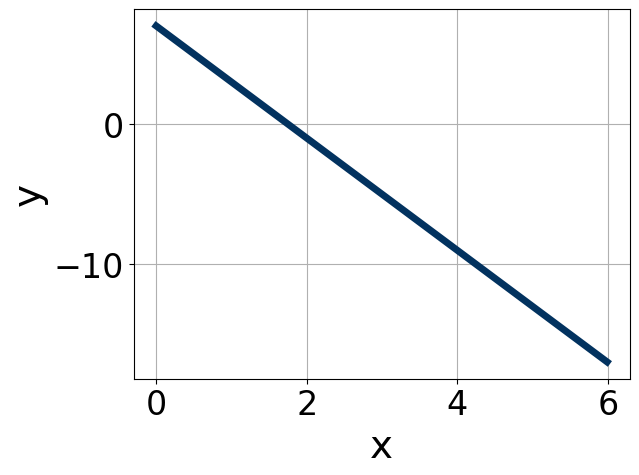
\includegraphics[width=0.5\textwidth]{../Figures/MA_8_F_1_2_graphP.png}
\end{center}


The solution is yes, the graph is linear., which is option A.

\begin{enumerate}[label=\Alph*.]
\item Yes, the graph is linear

* Correct! The graph has a constant rate of change and is thus a linear function.
\item No, the graph is not linear.

A linear function has a constant rate of growth. As $x$ increases/decreases, $y$ increases/decreases at the same rate. The graph in this example does have a constant rate of change.
\end{enumerate}


\textbf{General Comment:} The equation graphed was -4(x -3)-5. A linear function has a constant rate of growth. This means that as $x$ increases or decreases, $y$ increase or decreases at the same rate. For example, $x^2$ is NOT a linear function. As $x$ increases, the $y$ increases faster and faster. From $x=1$ to $x=2$, the $y$ increases by 3. From $x=2$ to $x=3$, the $y$ increases by 5. From $x=3$ to $x=4$, the $y$ increases by 7. A linear function would have the same change in $y$ for any change in $x$.
}
\litem{
Is the following relation a function?


\begin{tabular}{c|c}
x &y\tabularnewline \hline
3 &-3.46\tabularnewline \hline
4 &-4.0\tabularnewline \hline
5 &-4.47\tabularnewline \hline
6 &-4.9\tabularnewline \hline
7 &-5.29\tabularnewline \hline
8 &-5.66\tabularnewline \hline
9 &-6.0\end{tabular}The solution is Yes, which is option A.

\begin{enumerate}[label=\Alph*.]
\item Yes

* Correct! Every $x$-value has exactly one output.
\item No

For a relation to be a function, every $x$-value needs exactly one output. That means for a relation to NOT be a function, we would need one $x$-value that has two or more different outputs.
\end{enumerate}


\textbf{General Comment:} For a relation to be a function, every $x$-value needs exactly one output.
}
\litem{
Is the equation below a linear function?
\[ f(x) = -5(x -1)-2 \]The solution is yes, the graph is linear., which is option A.

\begin{enumerate}[label=\Alph*.]
\item Yes, the equation is linear

* Correct! The equation is a degree-1 polynomial and is thus a linear function.
\item No, the equation is not linear.

A linear function is a degree-1 polynomial. Polynomial equations have all variables with positive integer exponents.
\end{enumerate}


\textbf{General Comment:} The equation graphed was -5(x -1)-2. A linear function is a degree-1 polynomial. Polynomial equations have all variables with positive integer exponents, like $f(x) = 3x^2-2x+4$. Square root and cube root functions have rational exponents (1/2 and 1/3).
}
\litem{
Is the following relation a linear function?


\begin{tabular}{c|c}
x &y\tabularnewline \hline
3 &-18\tabularnewline \hline
4 &-32\tabularnewline \hline
5 &-50\tabularnewline \hline
6 &-72\tabularnewline \hline
7 &-72\tabularnewline \hline
6 &18\tabularnewline \hline
5 &32\end{tabular}The solution is No, which is option B.

\begin{enumerate}[label=\Alph*.]
\item Yes

Notice how one $x$-value has two separate outputs? For a relation to be a function, every $x$-value needs exactly one output.
\item No

* Correct! An $x$-value has two separate outputs and thus this relation is not a function, let alone a linear function.
\end{enumerate}


\textbf{General Comment:} For a relation to be a linear function, every $x$-value needs exactly one output AND there needs to be a constant rate of growth (as $x$ increases/decreases, $y$ increases/decreases at the same rate).
}
\litem{
Is the graph below a linear function?

\begin{center}
    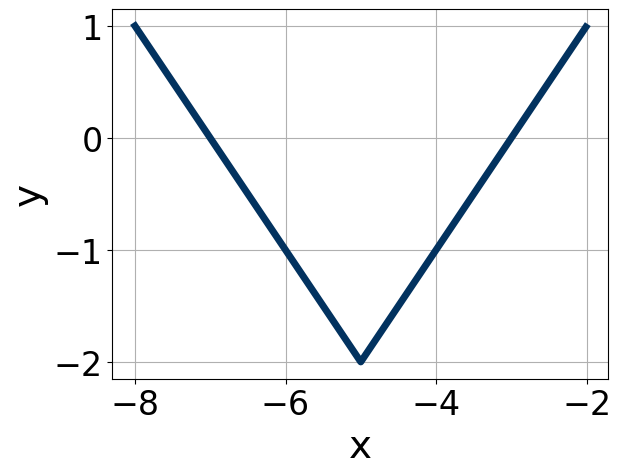
\includegraphics[width=0.5\textwidth]{../Figures/MA_8_F_1_2_graphQ.png}
\end{center}


The solution is no, the graph is not linear., which is option B.

\begin{enumerate}[label=\Alph*.]
\item Yes, the graph is linear

A linear function has a constant rate of growth. As $x$ increases/decreases, $y$ increases/decreases at the same rate. The graph in this example does not have a constant rate of change.
\item No, the graph is not linear.

* Correct! The graph does not have a constant rate of change and thus is not a linear function.
\end{enumerate}


\textbf{General Comment:} The equation graphed was 1|x + 5|-2. A linear function has a constant rate of growth. This means that as $x$ increases or decreases, $y$ increase or decreases at the same rate. For example, $x^2$ is NOT a linear function. As $x$ increases, the $y$ increases faster and faster. From $x=1$ to $x=2$, the $y$ increases by 3. From $x=2$ to $x=3$, the $y$ increases by 5. From $x=3$ to $x=4$, the $y$ increases by 7. A linear function would have the same change in $y$ for any change in $x$.
}
\litem{
Is the following relation a function?


\begin{tabular}{c|c}
x &y\tabularnewline \hline
2 &1.26\tabularnewline \hline
3 &1.44\tabularnewline \hline
4 &1.59\tabularnewline \hline
5 &1.71\tabularnewline \hline
6 &1.82\tabularnewline \hline
7 &1.91\tabularnewline \hline
8 &2.0\end{tabular}The solution is Yes, which is option A.

\begin{enumerate}[label=\Alph*.]
\item Yes

* Correct! Every $x$-value has exactly one output.
\item No

For a relation to be a function, every $x$-value needs exactly one output. That means for a relation to NOT be a function, we would need one $x$-value that has two or more different outputs.
\end{enumerate}


\textbf{General Comment:} For a relation to be a function, every $x$-value needs exactly one output.
}
\litem{
Is the equation below a linear function?
\[ f(x) = -3(x + 3)^4+1 \]The solution is no, the equation is not linear., which is option B.

\begin{enumerate}[label=\Alph*.]
\item Yes, the equation is linear

A linear equation is a degree-1 polynomial. -3(x + 3)^4+1 is a degree-4 polynomial
\item No, the equation is not linear.

* Correct! -3(x + 3)^4+1 is not a degree-1 polynomial.
\end{enumerate}


\textbf{General Comment:} The equation graphed was -3(x + 3)^4+1. A linear function is a degree-1 polynomial. Polynomial equations have all variables with positive integer exponents, like $f(x) = 3x^2-2x+4$. Square root and cube root functions have rational exponents (1/2 and 1/3).
}
\litem{
Is the following relation a linear function?


\begin{tabular}{c|c}
x &y\tabularnewline \hline
2 &-4.24\tabularnewline \hline
3 &-5.2\tabularnewline \hline
4 &-6.0\tabularnewline \hline
5 &-6.71\tabularnewline \hline
6 &-6.71\tabularnewline \hline
5 &4.24\tabularnewline \hline
4 &5.2\end{tabular}The solution is No, which is option B.

\begin{enumerate}[label=\Alph*.]
\item Yes

Notice how one $x$-value has two separate outputs? For a relation to be a function, every $x$-value needs exactly one output.
\item No

* Correct! An $x$-value has two separate outputs and thus this relation is not a function, let alone a linear function.
\end{enumerate}


\textbf{General Comment:} For a relation to be a linear function, every $x$-value needs exactly one output AND there needs to be a constant rate of growth (as $x$ increases/decreases, $y$ increases/decreases at the same rate).
}
\litem{
Is the graph below a linear function?

\begin{center}
    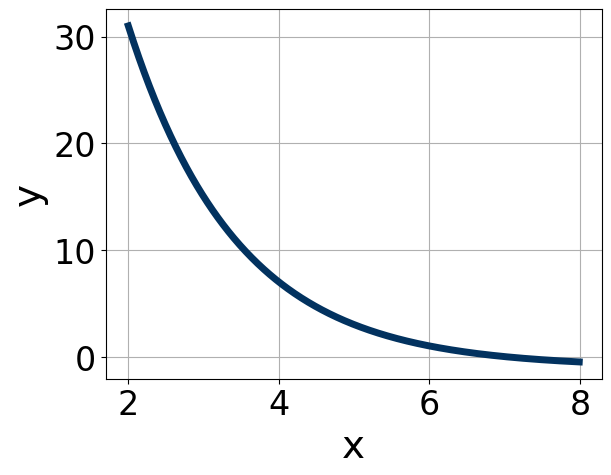
\includegraphics[width=0.5\textwidth]{../Figures/MA_8_F_1_2_graphR.png}
\end{center}


The solution is no, the graph is not linear., which is option B.

\begin{enumerate}[label=\Alph*.]
\item Yes, the graph is linear

A linear function has a constant rate of growth. As $x$ increases/decreases, $y$ increases/decreases at the same rate. The graph in this example does not have a constant rate of change.
\item No, the graph is not linear.

* Correct! The graph does not have a constant rate of change and thus is not a linear function.
\end{enumerate}


\textbf{General Comment:} The equation graphed was 4 \left( \dfrac{1}{2} \right)^{x-5}-1. A linear function has a constant rate of growth. This means that as $x$ increases or decreases, $y$ increase or decreases at the same rate. For example, $x^2$ is NOT a linear function. As $x$ increases, the $y$ increases faster and faster. From $x=1$ to $x=2$, the $y$ increases by 3. From $x=2$ to $x=3$, the $y$ increases by 5. From $x=3$ to $x=4$, the $y$ increases by 7. A linear function would have the same change in $y$ for any change in $x$.
}
\litem{
Is the following relation a function?
\[ (1, 4), (2, 16), (3, 36), (4, 64), (5, 64), (4, -4), (3, -16) \]The solution is No, which is option B.

\begin{enumerate}[label=\Alph*.]
\item Yes

Notice how one $x$-value has two separate outputs? For a relation to be a function, every $x$-value needs exactly one output.
\item No

* Correct! An $x$-value has two separate outputs and thus this relation is not a function.
\end{enumerate}


\textbf{General Comment:} For a relation to be a function, every $x$-value needs exactly one output.
}
\litem{
Is the equation below a linear function?
\[ f(x) = -5(x + 1)+3 \]The solution is yes, the graph is linear., which is option A.

\begin{enumerate}[label=\Alph*.]
\item Yes, the equation is linear

* Correct! The equation is a degree-1 polynomial and is thus a linear function.
\item No, the equation is not linear.

A linear function is a degree-1 polynomial. Polynomial equations have all variables with positive integer exponents.
\end{enumerate}


\textbf{General Comment:} The equation graphed was -5(x + 1)+3. A linear function is a degree-1 polynomial. Polynomial equations have all variables with positive integer exponents, like $f(x) = 3x^2-2x+4$. Square root and cube root functions have rational exponents (1/2 and 1/3).
}
\litem{
Is the following relation a linear function?


\begin{tabular}{c|c}
x &y\tabularnewline \hline
-1 &-5\tabularnewline \hline
0 &1\tabularnewline \hline
1 &7\tabularnewline \hline
2 &13\tabularnewline \hline
3 &19\tabularnewline \hline
4 &25\tabularnewline \hline
5 &31\end{tabular}The solution is Yes, which is option A.

\begin{enumerate}[label=\Alph*.]
\item Yes

* Correct! As $x$ increases/decreases, $y$ increases/decreases at the same rate.
\item No

A linear function has a constant rate of growth. As $x$ increases/decreases, $y$ increases/decreases at the same rate.
\end{enumerate}


\textbf{General Comment:} For a relation to be a linear function, every $x$-value needs exactly one output AND there needs to be a constant rate of growth (as $x$ increases/decreases, $y$ increases/decreases at the same rate).
}
\litem{
Is the graph below a linear function?

\begin{center}
    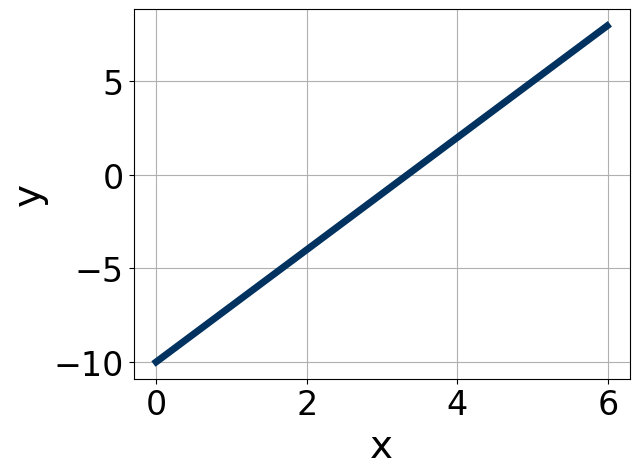
\includegraphics[width=0.5\textwidth]{../Figures/MA_8_F_1_2_graphS.png}
\end{center}


The solution is yes, the graph is linear., which is option A.

\begin{enumerate}[label=\Alph*.]
\item Yes, the graph is linear

* Correct! The graph has a constant rate of change and is thus a linear function.
\item No, the graph is not linear.

A linear function has a constant rate of growth. As $x$ increases/decreases, $y$ increases/decreases at the same rate. The graph in this example does have a constant rate of change.
\end{enumerate}


\textbf{General Comment:} The equation graphed was 3(x -3)-1. A linear function has a constant rate of growth. This means that as $x$ increases or decreases, $y$ increase or decreases at the same rate. For example, $x^2$ is NOT a linear function. As $x$ increases, the $y$ increases faster and faster. From $x=1$ to $x=2$, the $y$ increases by 3. From $x=2$ to $x=3$, the $y$ increases by 5. From $x=3$ to $x=4$, the $y$ increases by 7. A linear function would have the same change in $y$ for any change in $x$.
}
\litem{
Is the following relation a function?


\begin{tabular}{c|c}
x &y\tabularnewline \hline
1 &-1\tabularnewline \hline
2 &-4\tabularnewline \hline
3 &-9\tabularnewline \hline
4 &-16\tabularnewline \hline
5 &16\tabularnewline \hline
4 &1\tabularnewline \hline
3 &4\end{tabular}The solution is No, which is option B.

\begin{enumerate}[label=\Alph*.]
\item Yes

Notice how one $x$-value has two separate outputs? For a relation to be a function, every $x$-value needs exactly one output.
\item No

* Correct! An $x$-value has two separate outputs and thus this relation is not a function.
\end{enumerate}


\textbf{General Comment:} For a relation to be a function, every $x$-value needs exactly one output.
}
\litem{
Is the equation below a linear function?
\[ f(x) = 2(x -2)+2 \]The solution is yes, the graph is linear., which is option A.

\begin{enumerate}[label=\Alph*.]
\item Yes, the equation is linear

* Correct! The equation is a degree-1 polynomial and is thus a linear function.
\item No, the equation is not linear.

A linear function is a degree-1 polynomial. Polynomial equations have all variables with positive integer exponents.
\end{enumerate}


\textbf{General Comment:} The equation graphed was 2(x -2)+2. A linear function is a degree-1 polynomial. Polynomial equations have all variables with positive integer exponents, like $f(x) = 3x^2-2x+4$. Square root and cube root functions have rational exponents (1/2 and 1/3).
}
\litem{
Is the following relation a linear function?


\begin{tabular}{c|c}
x &y\tabularnewline \hline
-2 &-7\tabularnewline \hline
-1 &-1\tabularnewline \hline
0 &5\tabularnewline \hline
1 &11\tabularnewline \hline
2 &17\tabularnewline \hline
3 &23\tabularnewline \hline
4 &29\end{tabular}The solution is Yes, which is option A.

\begin{enumerate}[label=\Alph*.]
\item Yes

* Correct! As $x$ increases/decreases, $y$ increases/decreases at the same rate.
\item No

A linear function has a constant rate of growth. As $x$ increases/decreases, $y$ increases/decreases at the same rate.
\end{enumerate}


\textbf{General Comment:} For a relation to be a linear function, every $x$-value needs exactly one output AND there needs to be a constant rate of growth (as $x$ increases/decreases, $y$ increases/decreases at the same rate).
}
\litem{
Is the graph below a linear function?

\begin{center}
    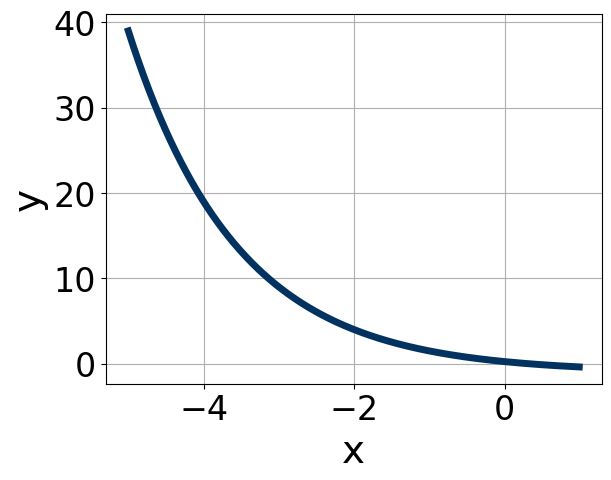
\includegraphics[width=0.5\textwidth]{../Figures/MA_8_F_1_2_graphT.png}
\end{center}


The solution is no, the graph is not linear., which is option B.

\begin{enumerate}[label=\Alph*.]
\item Yes, the graph is linear

A linear function has a constant rate of growth. As $x$ increases/decreases, $y$ increases/decreases at the same rate. The graph in this example does not have a constant rate of change.
\item No, the graph is not linear.

* Correct! The graph does not have a constant rate of change and thus is not a linear function.
\end{enumerate}


\textbf{General Comment:} The equation graphed was 5 \left( \dfrac{1}{2} \right)^{x--2}-1. A linear function has a constant rate of growth. This means that as $x$ increases or decreases, $y$ increase or decreases at the same rate. For example, $x^2$ is NOT a linear function. As $x$ increases, the $y$ increases faster and faster. From $x=1$ to $x=2$, the $y$ increases by 3. From $x=2$ to $x=3$, the $y$ increases by 5. From $x=3$ to $x=4$, the $y$ increases by 7. A linear function would have the same change in $y$ for any change in $x$.
}
\litem{
Is the following relation a function?


\begin{tabular}{c|c}
x &y\tabularnewline \hline
1 &4.0\tabularnewline \hline
2 &8.0\tabularnewline \hline
3 &16.0\tabularnewline \hline
4 &32.0\tabularnewline \hline
5 &64.0\tabularnewline \hline
6 &128.0\tabularnewline \hline
7 &256.0\end{tabular}The solution is Yes, which is option A.

\begin{enumerate}[label=\Alph*.]
\item Yes

* Correct! Every $x$-value has exactly one output.
\item No

For a relation to be a function, every $x$-value needs exactly one output. That means for a relation to NOT be a function, we would need one $x$-value that has two or more different outputs.
\end{enumerate}


\textbf{General Comment:} For a relation to be a function, every $x$-value needs exactly one output.
}
\litem{
Is the equation below a linear function?
\[ f(x) = {-4}\sqrt[3]{7x + 6}-3 \]The solution is no, the equation is not linear., which is option B.

\begin{enumerate}[label=\Alph*.]
\item Yes, the equation is linear

A linear equation is a degree-1 polynomial. {-4}\sqrt[3]{7x + 6}-3 is a cube root function
\item No, the equation is not linear.

* Correct! {-4}\sqrt[3]{7x + 6}-3 is not a degree-1 polynomial.
\end{enumerate}


\textbf{General Comment:} The equation graphed was {-4}\sqrt[3]{7x + 6}-3. A linear function is a degree-1 polynomial. Polynomial equations have all variables with positive integer exponents, like $f(x) = 3x^2-2x+4$. Square root and cube root functions have rational exponents (1/2 and 1/3).
}
\litem{
Is the following relation a linear function?


\begin{tabular}{c|c}
x &y\tabularnewline \hline
1 &2.0\tabularnewline \hline
2 &2.83\tabularnewline \hline
3 &-2.83\tabularnewline \hline
2 &-2.0\tabularnewline \hline
1 &-2.83\tabularnewline \hline
0 &-3.46\tabularnewline \hline
-1 &-4.0\end{tabular}The solution is No, which is option B.

\begin{enumerate}[label=\Alph*.]
\item Yes

Notice how one $x$-value has two separate outputs? For a relation to be a function, every $x$-value needs exactly one output.
\item No

* Correct! An $x$-value has two separate outputs and thus this relation is not a function, let alone a linear function.
\end{enumerate}


\textbf{General Comment:} For a relation to be a linear function, every $x$-value needs exactly one output AND there needs to be a constant rate of growth (as $x$ increases/decreases, $y$ increases/decreases at the same rate).
}
\litem{
Is the graph below a linear function?

\begin{center}
    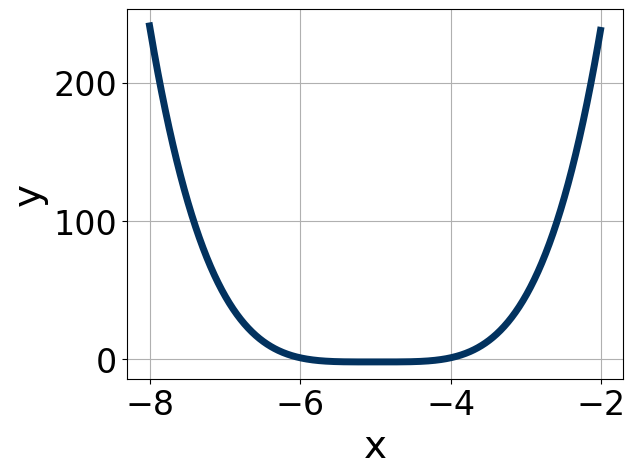
\includegraphics[width=0.5\textwidth]{../Figures/MA_8_F_1_2_graphU.png}
\end{center}


The solution is no, the graph is not linear., which is option B.

\begin{enumerate}[label=\Alph*.]
\item Yes, the graph is linear

A linear function has a constant rate of growth. As $x$ increases/decreases, $y$ increases/decreases at the same rate. The graph in this example does not have a constant rate of change.
\item No, the graph is not linear.

* Correct! The graph does not have a constant rate of change and thus is not a linear function.
\end{enumerate}


\textbf{General Comment:} The equation graphed was 3(x + 5)^4-2. A linear function has a constant rate of growth. This means that as $x$ increases or decreases, $y$ increase or decreases at the same rate. For example, $x^2$ is NOT a linear function. As $x$ increases, the $y$ increases faster and faster. From $x=1$ to $x=2$, the $y$ increases by 3. From $x=2$ to $x=3$, the $y$ increases by 5. From $x=3$ to $x=4$, the $y$ increases by 7. A linear function would have the same change in $y$ for any change in $x$.
}
\litem{
Is the following relation a function?
\[ (3, -27), (4, -48), (5, -75), (6, 75), (5, 27), (4, 48), (3, 75) \]The solution is No, which is option B.

\begin{enumerate}[label=\Alph*.]
\item Yes

Notice how one $x$-value has two separate outputs? For a relation to be a function, every $x$-value needs exactly one output.
\item No

* Correct! An $x$-value has two separate outputs and thus this relation is not a function.
\end{enumerate}


\textbf{General Comment:} For a relation to be a function, every $x$-value needs exactly one output.
}
\litem{
Is the equation below a linear function?
\[ f(x) = 2(x + 4)+1 \]The solution is yes, the graph is linear., which is option A.

\begin{enumerate}[label=\Alph*.]
\item Yes, the equation is linear

* Correct! The equation is a degree-1 polynomial and is thus a linear function.
\item No, the equation is not linear.

A linear function is a degree-1 polynomial. Polynomial equations have all variables with positive integer exponents.
\end{enumerate}


\textbf{General Comment:} The equation graphed was 2(x + 4)+1. A linear function is a degree-1 polynomial. Polynomial equations have all variables with positive integer exponents, like $f(x) = 3x^2-2x+4$. Square root and cube root functions have rational exponents (1/2 and 1/3).
}
\litem{
Is the following relation a linear function?


\begin{tabular}{c|c}
x &y\tabularnewline \hline
3 &15\tabularnewline \hline
4 &20\tabularnewline \hline
5 &20\tabularnewline \hline
4 &-15\tabularnewline \hline
3 &-20\tabularnewline \hline
2 &-25\tabularnewline \hline
1 &-30\end{tabular}The solution is No, which is option B.

\begin{enumerate}[label=\Alph*.]
\item Yes

Notice how one $x$-value has two separate outputs? For a relation to be a function, every $x$-value needs exactly one output.
\item No

* Correct! An $x$-value has two separate outputs and thus this relation is not a function, let alone a linear function.
\end{enumerate}


\textbf{General Comment:} For a relation to be a linear function, every $x$-value needs exactly one output AND there needs to be a constant rate of growth (as $x$ increases/decreases, $y$ increases/decreases at the same rate).
}
\litem{
Is the graph below a linear function?

\begin{center}
    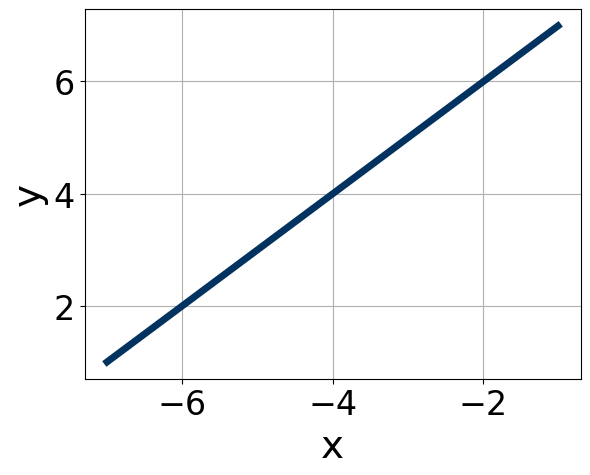
\includegraphics[width=0.5\textwidth]{../Figures/MA_8_F_1_2_graphV.png}
\end{center}


The solution is yes, the graph is linear., which is option A.

\begin{enumerate}[label=\Alph*.]
\item Yes, the graph is linear

* Correct! The graph has a constant rate of change and is thus a linear function.
\item No, the graph is not linear.

A linear function has a constant rate of growth. As $x$ increases/decreases, $y$ increases/decreases at the same rate. The graph in this example does have a constant rate of change.
\end{enumerate}


\textbf{General Comment:} The equation graphed was 1(x + 4)+4. A linear function has a constant rate of growth. This means that as $x$ increases or decreases, $y$ increase or decreases at the same rate. For example, $x^2$ is NOT a linear function. As $x$ increases, the $y$ increases faster and faster. From $x=1$ to $x=2$, the $y$ increases by 3. From $x=2$ to $x=3$, the $y$ increases by 5. From $x=3$ to $x=4$, the $y$ increases by 7. A linear function would have the same change in $y$ for any change in $x$.
}
\litem{
Is the following relation a function?


\begin{tabular}{c|c}
x &y\tabularnewline \hline
4 &-7.94\tabularnewline \hline
5 &-8.55\tabularnewline \hline
6 &-9.09\tabularnewline \hline
7 &-9.56\tabularnewline \hline
8 &-10.0\tabularnewline \hline
9 &-10.4\tabularnewline \hline
10 &-10.77\end{tabular}The solution is Yes, which is option A.

\begin{enumerate}[label=\Alph*.]
\item Yes

* Correct! Every $x$-value has exactly one output.
\item No

For a relation to be a function, every $x$-value needs exactly one output. That means for a relation to NOT be a function, we would need one $x$-value that has two or more different outputs.
\end{enumerate}


\textbf{General Comment:} For a relation to be a function, every $x$-value needs exactly one output.
}
\litem{
Is the equation below a linear function?
\[ f(x) = 5(x -5)-3 \]The solution is yes, the graph is linear., which is option A.

\begin{enumerate}[label=\Alph*.]
\item Yes, the equation is linear

* Correct! The equation is a degree-1 polynomial and is thus a linear function.
\item No, the equation is not linear.

A linear function is a degree-1 polynomial. Polynomial equations have all variables with positive integer exponents.
\end{enumerate}


\textbf{General Comment:} The equation graphed was 5(x -5)-3. A linear function is a degree-1 polynomial. Polynomial equations have all variables with positive integer exponents, like $f(x) = 3x^2-2x+4$. Square root and cube root functions have rational exponents (1/2 and 1/3).
}
\litem{
Is the following relation a linear function?


\begin{tabular}{c|c}
x &y\tabularnewline \hline
3 &-45\tabularnewline \hline
4 &-80\tabularnewline \hline
5 &80\tabularnewline \hline
4 &45\tabularnewline \hline
3 &80\tabularnewline \hline
2 &125\tabularnewline \hline
1 &180\end{tabular}The solution is No, which is option B.

\begin{enumerate}[label=\Alph*.]
\item Yes

Notice how one $x$-value has two separate outputs? For a relation to be a function, every $x$-value needs exactly one output.
\item No

* Correct! An $x$-value has two separate outputs and thus this relation is not a function, let alone a linear function.
\end{enumerate}


\textbf{General Comment:} For a relation to be a linear function, every $x$-value needs exactly one output AND there needs to be a constant rate of growth (as $x$ increases/decreases, $y$ increases/decreases at the same rate).
}
\litem{
Is the graph below a linear function?

\begin{center}
    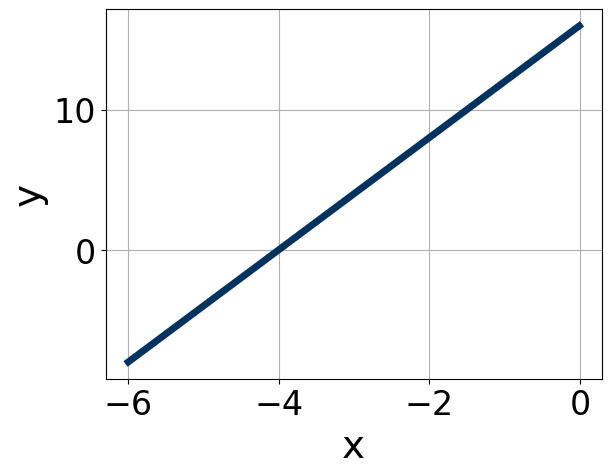
\includegraphics[width=0.5\textwidth]{../Figures/MA_8_F_1_2_graphW.png}
\end{center}


The solution is yes, the graph is linear., which is option A.

\begin{enumerate}[label=\Alph*.]
\item Yes, the graph is linear

* Correct! The graph has a constant rate of change and is thus a linear function.
\item No, the graph is not linear.

A linear function has a constant rate of growth. As $x$ increases/decreases, $y$ increases/decreases at the same rate. The graph in this example does have a constant rate of change.
\end{enumerate}


\textbf{General Comment:} The equation graphed was 4(x + 3)+4. A linear function has a constant rate of growth. This means that as $x$ increases or decreases, $y$ increase or decreases at the same rate. For example, $x^2$ is NOT a linear function. As $x$ increases, the $y$ increases faster and faster. From $x=1$ to $x=2$, the $y$ increases by 3. From $x=2$ to $x=3$, the $y$ increases by 5. From $x=3$ to $x=4$, the $y$ increases by 7. A linear function would have the same change in $y$ for any change in $x$.
}
\litem{
Is the following relation a function?


\begin{tabular}{c|c}
x &y\tabularnewline \hline
3 &-27\tabularnewline \hline
4 &-48\tabularnewline \hline
5 &-75\tabularnewline \hline
6 &-108\tabularnewline \hline
7 &-147\tabularnewline \hline
8 &-192\tabularnewline \hline
9 &-243\end{tabular}The solution is Yes, which is option A.

\begin{enumerate}[label=\Alph*.]
\item Yes

* Correct! Every $x$-value has exactly one output.
\item No

For a relation to be a function, every $x$-value needs exactly one output. That means for a relation to NOT be a function, we would need one $x$-value that has two or more different outputs.
\end{enumerate}


\textbf{General Comment:} For a relation to be a function, every $x$-value needs exactly one output.
}
\litem{
Is the equation below a linear function?
\[ f(x) = -5(x + 5)^4+2 \]The solution is no, the equation is not linear., which is option B.

\begin{enumerate}[label=\Alph*.]
\item Yes, the equation is linear

A linear equation is a degree-1 polynomial. -5(x + 5)^4+2 is a degree-4 polynomial
\item No, the equation is not linear.

* Correct! -5(x + 5)^4+2 is not a degree-1 polynomial.
\end{enumerate}


\textbf{General Comment:} The equation graphed was -5(x + 5)^4+2. A linear function is a degree-1 polynomial. Polynomial equations have all variables with positive integer exponents, like $f(x) = 3x^2-2x+4$. Square root and cube root functions have rational exponents (1/2 and 1/3).
}
\litem{
Is the following relation a linear function?


\begin{tabular}{c|c}
x &y\tabularnewline \hline
2 &6.3\tabularnewline \hline
3 &7.21\tabularnewline \hline
4 &7.94\tabularnewline \hline
5 &8.55\tabularnewline \hline
6 &9.09\tabularnewline \hline
7 &9.56\tabularnewline \hline
8 &10.0\end{tabular}The solution is No, which is option B.

\begin{enumerate}[label=\Alph*.]
\item Yes

A linear function has a constant rate of growth. As $x$ increases/decreases, $y$ increases/decreases at the same rate. The table in this example does have a constant rate of change.
\item No

* Correct! The table in this example does not have a constant rate of change. This relation is a float function.
\end{enumerate}


\textbf{General Comment:} For a relation to be a linear function, every $x$-value needs exactly one output AND there needs to be a constant rate of growth (as $x$ increases/decreases, $y$ increases/decreases at the same rate).
}
\litem{
Is the graph below a linear function?

\begin{center}
    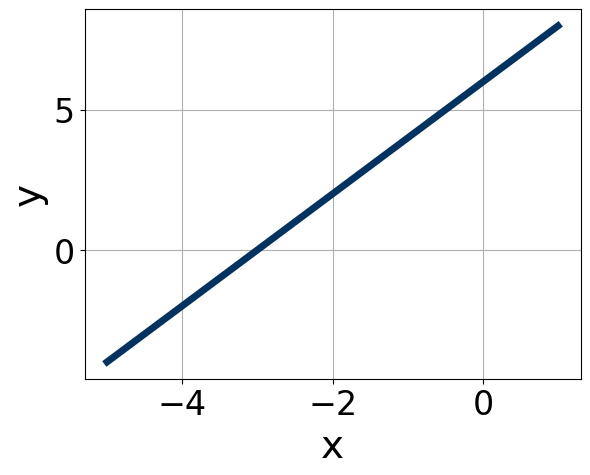
\includegraphics[width=0.5\textwidth]{../Figures/MA_8_F_1_2_graphX.png}
\end{center}


The solution is yes, the graph is linear., which is option A.

\begin{enumerate}[label=\Alph*.]
\item Yes, the graph is linear

* Correct! The graph has a constant rate of change and is thus a linear function.
\item No, the graph is not linear.

A linear function has a constant rate of growth. As $x$ increases/decreases, $y$ increases/decreases at the same rate. The graph in this example does have a constant rate of change.
\end{enumerate}


\textbf{General Comment:} The equation graphed was 2(x + 2)+2. A linear function has a constant rate of growth. This means that as $x$ increases or decreases, $y$ increase or decreases at the same rate. For example, $x^2$ is NOT a linear function. As $x$ increases, the $y$ increases faster and faster. From $x=1$ to $x=2$, the $y$ increases by 3. From $x=2$ to $x=3$, the $y$ increases by 5. From $x=3$ to $x=4$, the $y$ increases by 7. A linear function would have the same change in $y$ for any change in $x$.
}
\litem{
Is the following relation a function?
\[ (-4, -48), (-3, -27), (-2, -12), (-1, -3), (0, 0), (1, -3), (2, -12) \]The solution is Yes, which is option A.

\begin{enumerate}[label=\Alph*.]
\item Yes

* Correct! Every $x$-value has exactly one output.
\item No

For a relation to be a function, every $x$-value needs exactly one output. That means for a relation to NOT be a function, we would need one $x$-value that has two or more different outputs.
\end{enumerate}


\textbf{General Comment:} For a relation to be a function, every $x$-value needs exactly one output.
}
\litem{
Is the equation below a linear function?
\[ f(x) = 5(x -5)+2 \]The solution is yes, the graph is linear., which is option A.

\begin{enumerate}[label=\Alph*.]
\item Yes, the equation is linear

* Correct! The equation is a degree-1 polynomial and is thus a linear function.
\item No, the equation is not linear.

A linear function is a degree-1 polynomial. Polynomial equations have all variables with positive integer exponents.
\end{enumerate}


\textbf{General Comment:} The equation graphed was 5(x -5)+2. A linear function is a degree-1 polynomial. Polynomial equations have all variables with positive integer exponents, like $f(x) = 3x^2-2x+4$. Square root and cube root functions have rational exponents (1/2 and 1/3).
}
\litem{
Is the following relation a linear function?


\begin{tabular}{c|c}
x &y\tabularnewline \hline
1 &-2\tabularnewline \hline
2 &-4\tabularnewline \hline
3 &-4\tabularnewline \hline
2 &2\tabularnewline \hline
1 &4\tabularnewline \hline
0 &6\tabularnewline \hline
-1 &8\end{tabular}The solution is No, which is option B.

\begin{enumerate}[label=\Alph*.]
\item Yes

Notice how one $x$-value has two separate outputs? For a relation to be a function, every $x$-value needs exactly one output.
\item No

* Correct! An $x$-value has two separate outputs and thus this relation is not a function, let alone a linear function.
\end{enumerate}


\textbf{General Comment:} For a relation to be a linear function, every $x$-value needs exactly one output AND there needs to be a constant rate of growth (as $x$ increases/decreases, $y$ increases/decreases at the same rate).
}
\litem{
Is the graph below a linear function?

\begin{center}
    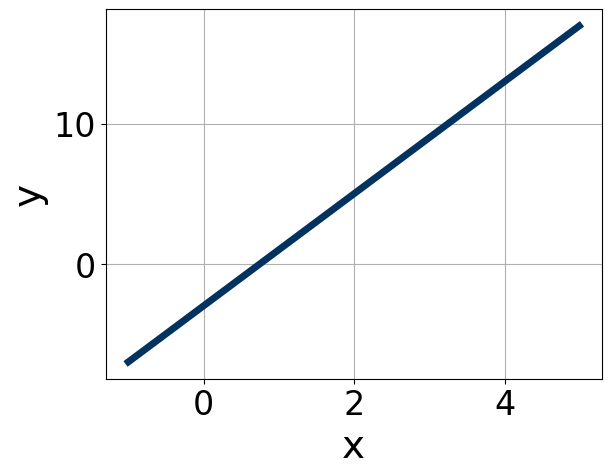
\includegraphics[width=0.5\textwidth]{../Figures/MA_8_F_1_2_graphY.png}
\end{center}


The solution is yes, the graph is linear., which is option A.

\begin{enumerate}[label=\Alph*.]
\item Yes, the graph is linear

* Correct! The graph has a constant rate of change and is thus a linear function.
\item No, the graph is not linear.

A linear function has a constant rate of growth. As $x$ increases/decreases, $y$ increases/decreases at the same rate. The graph in this example does have a constant rate of change.
\end{enumerate}


\textbf{General Comment:} The equation graphed was 4(x -2)+5. A linear function has a constant rate of growth. This means that as $x$ increases or decreases, $y$ increase or decreases at the same rate. For example, $x^2$ is NOT a linear function. As $x$ increases, the $y$ increases faster and faster. From $x=1$ to $x=2$, the $y$ increases by 3. From $x=2$ to $x=3$, the $y$ increases by 5. From $x=3$ to $x=4$, the $y$ increases by 7. A linear function would have the same change in $y$ for any change in $x$.
}
\litem{
Is the following relation a function?
\[ (4, 0.12), (5, 0.06), (6, 0.03), (7, 0.02), (8, 0.01), (9, 0.0), (10, 0.0) \]The solution is Yes, which is option A.

\begin{enumerate}[label=\Alph*.]
\item Yes

* Correct! Every $x$-value has exactly one output.
\item No

For a relation to be a function, every $x$-value needs exactly one output. That means for a relation to NOT be a function, we would need one $x$-value that has two or more different outputs.
\end{enumerate}


\textbf{General Comment:} For a relation to be a function, every $x$-value needs exactly one output.
}
\litem{
Is the equation below a linear function?
\[ f(x) = 4(x + 5)-1 \]The solution is yes, the graph is linear., which is option A.

\begin{enumerate}[label=\Alph*.]
\item Yes, the equation is linear

* Correct! The equation is a degree-1 polynomial and is thus a linear function.
\item No, the equation is not linear.

A linear function is a degree-1 polynomial. Polynomial equations have all variables with positive integer exponents.
\end{enumerate}


\textbf{General Comment:} The equation graphed was 4(x + 5)-1. A linear function is a degree-1 polynomial. Polynomial equations have all variables with positive integer exponents, like $f(x) = 3x^2-2x+4$. Square root and cube root functions have rational exponents (1/2 and 1/3).
}
\litem{
Is the following relation a linear function?


\begin{tabular}{c|c}
x &y\tabularnewline \hline
2 &-0.25\tabularnewline \hline
3 &-0.12\tabularnewline \hline
4 &-0.06\tabularnewline \hline
5 &-0.03\tabularnewline \hline
6 &-0.02\tabularnewline \hline
7 &-0.01\tabularnewline \hline
8 &-0.0\end{tabular}The solution is No, which is option B.

\begin{enumerate}[label=\Alph*.]
\item Yes

A linear function has a constant rate of growth. As $x$ increases/decreases, $y$ increases/decreases at the same rate. The table in this example does have a constant rate of change.
\item No

* Correct! The table in this example does not have a constant rate of change. This relation is a float function.
\end{enumerate}


\textbf{General Comment:} For a relation to be a linear function, every $x$-value needs exactly one output AND there needs to be a constant rate of growth (as $x$ increases/decreases, $y$ increases/decreases at the same rate).
}
\end{enumerate}

\end{document}